\chapter{Di-$b$-jet Search: Limit Setting}
\label{sec:lim}

%Specifically, what was found was that the probability of obtaining a data-set with an excess similar to the one observed
%under the assumption that there is new physics was above a certain threshold.
%This lead to the conclusion that there is no evidence of BSM physics in the di-$b$-jet spectra.

In Chapter~\ref{sec:bkg} it was shown that there is no evidence of new physics in the di-$b$-jet spectra considered.
However, it is also useful to quantify what this result means in the context
of the signal models that we are searching for.
Specifically, we can estimate the degree of belief that a signal model is true given the di-$b$-jet spectra that have been observed.
If the degree of belief of a specific model is less than a certain threshold it is said that this model is excluded.
This process is known as limit setting.

In this Chapter:
Section~\ref{sec:lim-strat} will describe the limit setting strategy used,
Section~\ref{sec:lim-syst} will discuss the systematic uncertainties considered
and in Section~\ref{sec:lim-summer} and Section~\ref{sec:lim-full} presents the details and
the results of the limit setting procedure for the \summer{} and \lm{} data-sets respectively.

\section{Bayesian Limits}
\label{sec:lim-strat}

In this analysis a Bayesian limit setting approach is used~\cite{lim-bayes}.
For limit setting, one considers a hypothesis that the di-$b$-jet events are produced by a combination of 
the QCD background, which has been modelled by the background estimates described in the previous chapter,
and some new physics process 
which produces $\mu$ events according to some template shape in~\mjj.
This signal plus background hypothesis is denoted by the symbol $H_\mu$.

Now let us consider this hypothesis in the context of the data, denoted by $D$,
which in this case is one of our observed di-$b$-jet spectra.
For the hypothesis, $H_\mu$, the probability of producing the data is known as the ``likelihood''.
If, in each~\mjj~bin, the model predicts
$s_i(\mu)$ signal events, $b_i$ background events and $n_i$ events were observed in data.
Then, by only considering statistical uncertainties, the likelihood for a given value of $\mu$ is given by
\begin{equation}
  \Like (\mu,D) = P(D \mid \mu) =  \Pi_i \frac{(s_i(\mu)+b_i)^{n_i}~e^{-(s_i(\mu)+b_i)}}{n_i!}
  \label{eqn:lim-like}
\end{equation}
where the product is over all~\mjj~bins and
the notation $P(A \mid B)$ represents the probability of event $A$ occurring
given the event $B$ has occurred.

\noindent
Then, one can employ Bayes' theorem which states that
\begin{equation}
  P(A \mid B) = \frac{P(B \mid A) \, P(A)}{P(B)}
\end{equation}
to obtain the probability density function of $\mu$ given the observed di-$b$-jet spectrum,
\begin{equation}
  P(\mu \mid D) = \frac{ P(D \mid \mu) \, \Pi( \mu ) }{ \Pi( D ) }
  \label{eq:lim-conf_statOnly}
\end{equation}
This quantity, known as the posterior, is an expression of the degree of belief in the hypothesis
$H_\mu$ for any particular value of $\mu$.
The $\Pi( \mu )$ term in the posterior %Equation~\ref{eq:lim-conf_statOnly}
is called the signal prior
and gives the probability density of $\mu$ before the experiment took place.
A prior flat with respect to $\mu$ is used
\footnote{Flat from $\mu$ = 0 to the value of $\mu$ where the
likelihood has fallen to $10^{-5}$ of the optimal likelihood value.}
which represents ignorance to the size of the signal before the experiment.
The $\Pi(D)$ term does not depend on $\mu$ and as such can be considered as a normalisation term.

However, to accurately represent a true degree of belief in a model one must consider the systematic uncertainties,
which are uncertainties in the values of $b_i$ and $s_i$ in Equation~\ref{eqn:lim-like}.
The systematic uncertainties considered in this analysis are listed below in Section~\ref{sec:lim-syst}.
The systematic uncertainties are incorporated by explicitly considering $s_i$ and $b_i$ as a
function of the parameters which have a systematic uncertainty,
the parameters used are known as nuisance parameters.
For example, the number of signal events, $s_i$, is linearly dependant on luminosity ($L$) such that $s_i(L) \propto L$.
Here luminosity is an example of a nuisance parameter.

Therefore the likelihood becomes a function of the nuisance parameters
\begin{equation}
  \Like (\mu,D,\vec{\theta}) = P(D \mid \mu, \vec{\theta} ) =  \Pi_i \frac{(s_i(\mu,\vec{\theta})+b_i(\vec{\theta})^{n_i}~e^{-(s_i(\mu,\vec{\theta})+b_i(\vec{\theta}))}}{n_i!}
\end{equation}
where $\vec{\theta}$ represents the set of nuisance parameters.
The effect of the systematic uncertainties are then propagated to the posterior. %Equation~\ref{eq:lim-conf_statOnly}.
To do this a prior is introduced for each the nuisance parameters, given by $\Pi(\vec{\theta})$,
that describes the prior probability distribution of the nuisance parameters.
Then, by integrating over the nuisance parameters,
one obtains the probability density function for $\mu$ that includes the systematic uncertainties
\begin{equation}
  P(\mu \mid D) \propto \int d \vec{\theta} \, \Like (\mu, D, \vec{\theta} ) \, \Pi( \mu )  \, \Pi(\vec{\theta})
  \label{eq:lim-conf_syst}
\end{equation}
One can calculate the likelihoods for the data,
perform the integral over nuisance parameters
and then normalise to calculate the probability density of $\mu$
\footnote{This integral is performed using a Markov chain Monte-Carlo using the Bayesian Analysis Toolkit.
 Full details on the implementation can be found here~\cite{det-thesis_kate}.}.

Using the posterior calculated from Equation~\ref{eq:lim-conf_syst},
the 95\% credibility level upper limit of $\mu$, denoted by $\mu_{up}\,$,
is calculated using the expression
\begin{equation}
\int_0^{\mu_{up}} P(\mu \mid D)~=~0.95
\end{equation}
The 95\% credibility upper limit defines an interval ($0 < \mu < \mu_{up}$)
that will contain the true value of $\mu$ with 95\% probability.
Any model under the hypothesis $H_{\mu}$ that predicts a $\mu$
value outside of this region is said to be excluded at the 95\% credibility level.

In the di-$b$-jet analysis limits are set using the benchmark signal model templates for a range of mass points,
%the models and mass points considered
as described in Section~\ref{sec:evt-s+b}.
The limits are presented in terms of the product of cross-section, detector acceptance and tagging efficiency,
$\sigma\,\text{x}\,\mathit{A}\,\text{x}\,\epsilon$,
which is related to the parameter $\mu$ used in the limit setting description
\footnote{
  Specifically $\mu$=$\sigma/L$, where $L$ is the luminosity.
  $\mathit{A}$ and $\epsilon$ have been measured in Section~\ref{sec:evt-sel-acc}.
}.
Further to this
many BSM models predicting a narrow resonance
not explicitly considered by this analysis
can be approximated by a Gaussian distribution,
if low-mass off-shell tails and non-perturbative effects are neglected.
Therefore, limits are set using a signal template with a Gaussian shape,
which can be reinterpreted for a wider range of models.
  
The di-$b$-jet analysis will present two limits, which is typical of searches at ATLAS.
The first is the observed limit, which is the limit using the observed di-$b$-spectra as $D$, which was described above.
The second is the expected limit under the assumption that there is no signal in the di-$b$-jet spectrum.
To calculate the expected limit the procedure is performed where $D$ is replaced by pseudo-experiments
created by varying the background estimate within the systematic uncertainties.
This process can be done for many pseudo-experiments; the median upper limit found gives the expected limit
and the 68\% and 95\% percentiles give the 1 and 2 $\sigma$ uncertainty bands on the expected limit.

In this analysis the Bayesian approach for limit setting is used,
while there is a widely used alternative known as the frequentist approach.
The Bayesian approach defines a credibility interval using the probability (or degree of belief) in a hypothesis given the observed data ( $P(\mu \mid D)$ ).
On the other hand, the frequentist approach calculates the probability (or fraction of trials)
of obtaining the data assuming a given signal model is true ( $P(D \mid \mu)$ ) and rejects models that produce a low probability~\cite{lim-cowan}.
%Bayesian limits are used for two reasons,
%firstly, it has been argued that the Bayesian approach is a more intuitive statistical interpretation of the limits.
%Secondly, the Bayesian approach has been used in other di-jet search analyses at ATLAS~\cite{dijet-mori16_paper}
%which allows for comparable results and shared development of computational framework.
Both approaches are valid and logically consistent,
but it is important that one states clearly which approach is being taken
\footnote{As a side note the BumpHunter $p$-value uses the frequentist approach to calculate a $p$-value.}.

\section{Description of Systematic Uncertainties}
\label{sec:lim-syst}

As discussed in the previous section,
systematic uncertainties are an important consideration in limit-setting.
They describe the uncertainty in the signal or background prediction
and are accounted for in the limit setting procedure through the inclusion of nuisance parameters.

The systematic uncertainties in the di-$b$-jet analysis considered are grouped into two categories~\cite{dibjet-ichep_conf}.
The first are
uncertainties on the signal~\mjj~templates used in the limit setting procedure.
Simulated Monte-Carlo signal templates are used,
hence a range of systematic uncertainties of the simulation are required.
The signal systematic uncertainties considered are:
\begin{itemize}[leftmargin=*]
\item\textbf{Jet Energy Scale, Jet Energy Resolution  and $b$-Jet Energy Scale} \hspace{1mm} (\textit{Signal}):\\
  Jet energy scale (JES) and jet energy resolution (JER) are uncertainties in the measurement of the jet energy,
  which causes on uncertainty of the width of the dijet mass signal templates.
  The JES and JER uncertainties used in this analysis were described in Section~\ref{sec:obj-jets_uncert}.
  In addition, there is also an additional $b$-jet energy scale ($b$JES) uncertainty which
  has been described in Section~\ref{sec:obj-bjets_bjes}.
  \vspace{0.5em}
\item\textbf{$b$-Tagging} \hspace{1mm} (\textit{Signal}):\\
  The $b$-tagging modelling in Monte-Carlo simulation is calibrated to data using measured $b$-tagging scale factors,
  the scale factors and associated uncertainties are discussed in Section~\ref{sec:obj-bjets_calib}.
  The uncertainty on $b$-tagging scale factor causes on uncertainty on the normalisation of each point in the dijet mass signal template.
  The $b$-tagging systematic uncertainty is large at high values of jet-\pT.%, and as such is the dominant uncertainty in this analysis.
  \vspace{0.5em}
\item\textbf{$b$-Jet Trigger} \hspace{1mm} (\textit{Signal}) - \lm{} data-set only:\\
  Similarly, when using the $b$-jet trigger,
  the online $b$-tagging efficiency is corrected to data using $b$-jet trigger scale factors.
  The $b$-jet trigger scale factors and relevant uncertainties are derived in Section~\ref{sec:trig-bjet_eff}.
  The uncertainty on the $b$-jet trigger scale factors cause an uncertainty on the normalisation of each point in the dijet mass signal template.
  This systematic uncertainty is only used in the \lm{} data-set, as this is the only data-set using a $b$-jet trigger.
  \vspace{0.5em}
\item\textbf{Luminosity} \hspace{1mm} (\textit{Signal}):\\
  The luminosity uncertainty is determined using the methodology outlined in~\cite{lim-syst_lumi}.
  %from van der Meer scans performed in August 2015 and May 2016.
  The luminosity uncertainties used are 2.9\% in the \summer{} data-set,
  2.2\% in the \lm{} data-set
  and 2.1\% in the \hm{} data-set.
  The uncertainty on luminosity causes an uncertainty on the normalisation of the dijet mass signal template.
  \vspace{0.5em}
\item\textbf{Parton Distribution Functions (PDFs) } \hspace{1mm}  (\textit{Signal}):\\
  The PDFs are important in calculating the cross-section of any process at the LHC.
  As shown in Section~\ref{sec:theo-qcd_pdf} there are uncertainties on the measurements of the PDFs,
  which causes an uncertainty in the signal template used.
  A flat 1\% uncertainty from the PDFs is considered,
  which has been found at previous dijet searches to conservatively cover
  the effect of the PDF uncertainties~\cite{dijet-mori16_paper}.
  The uncertainty on PDF causes is treated as an uncertainty on the normalisation of the dijet mass signal template.
  \vspace{0.5em}
\end{itemize}

The second group are systematic uncertainties of the background estimate.
As the background estimate is data-driven,
the large range of simulation modelling uncertainties considered for the signal model are not required.
The uncertainties on the background estimation model are:

\begin{itemize}[leftmargin=*]
\item \textbf{Fit Function Parameters} \hspace{1mm} (\textit{Background}):\\
  The choice of fit parameters is made by maximising the likelihood of the fit function with respect to our data-set.
  However, due to the statistical fluctuations in data the optimal parameters to describe
  the true background shape may not have been chosen.
  To estimate the uncertainty on the choice of parameters, pseudo-experiments are created by applying Poisson
  fluctuations to the background estimate and then running the background estimation fit procedure on the pseudo-experiments.
  The \textit{rms} of the difference between the nominal background estimate on data to those from the pseudo-experiments is
  taken as a symmetric uncertainty. \vspace{0.5em}
\item\textbf{Fit Function Choice}  \hspace{1mm} (\textit{Background}):\\
  A different background estimation can be obtained if a different fit function is chosen.
  To obtain a uncertainty on the choice of fit function an alternate function is considered,
  which is the dijet fit function with one extra degree of freedom than the nominal function.
  The alternate function is then used to fit to the pseudo-experiments described in the previous bullet point
  and the mean of the difference between the nominal and alternate functions is taken as a one-sided uncertainty.
  \vspace{0.5em}
\end{itemize}

\section{\summer{} Data-set Limits}
\label{sec:lim-summer}

Table~\ref{tab:lim-summer_syst} summarises the systematic uncertainties
on the signal template used in the \summer{} data-set at
three different values of dijet mass~\mjj.
Figure~\ref{fig:lim-summer_systBkg} shows the systematic uncertainties on the background estimate
for both $b$-tagging categories as a function of dijet mass,~\mjj.
%Reconstructed mass is defined as invariant mass of the two observed jets.
%$b$-tagging is the dominant systematic uncertainty for the full range of~\mjj.

\begin{table}[!htb]
  \centering
  \begin{tabular}{|c||c|c|c|c|c|c|}
    \hline
    \mjj   & \multicolumn{6}{c|}{Signal Systematic Uncertainties}                    \\ \cline{2-7} 
           & JES   & JER   & $b$JES  & $b$-Tagging ($\geq$1 / 2) & PDF & Lumi        \\
    \hline                                                                        
    1.5 TeV & 1.2\% & 1.0\% & 2.2\%   &        20\% / 10\%        & 1\% & 2.9\%       \\
    3 TeV   & 1.4\% & 0.7\% & 0.7\%   &        50\% / 60\%        & 1\% & 2.9\%       \\
    5 TeV   & 2.3\% & 0.3\% & 0.3\%   &        50\% / 70\%        & 1\% & 2.9\%       \\
    \hline
    % The background uncertainties
    %& \multicolumn{2}{c|}{Bkg. Uncert}             
    %&  Para. ($\geq$1 / 2)   & Func. ($\geq$1 / 2) 
    %                                               
    %&  1.3\%/0.0\%      & 0.3\%/0.0\%              
    %&  3.9\%/1.7\%      & 1.3\%/0.6\%           
    %&   22\%/ 17\%      & 7.5\%/5.1\%
  \end{tabular}
\caption[A table summarising the signal systematic uncertainties used in the \textit{Summer16+15} data-set.
    Jet Energy Scale (JES), Jet Energy Resolution (JER) and $b$-Jet Energy Scale ($b$JES) 
    are uncertainties on the dijet mass of a simulated event,
    whilst $b$-tagging, PDF and luminosity uncertainties are uncertainties on the simulated event weight.]
        {A table summarising the signal systematic uncertainties used in the \textit{Summer16+15} data-set.
          Jet Energy Scale (JES), Jet Energy Resolution (JER) and $b$-Jet Energy Scale ($b$JES)
          are uncertainties on the dijet mass of a simulated event,
          whilst $b$-tagging, PDF and luminosity uncertainties are uncertainties on simulated event weight.
          Values taken from~\cite{dibjet-ichep_int}.}
  \label{tab:lim-summer_syst}
  \end{table}

\begin{figure}[!ht]
  \begin{center}
    \captionsetup[subfigure]{aboveskip=0pt,justification=centering}
    \subcaptionbox{2 $b$-tag}{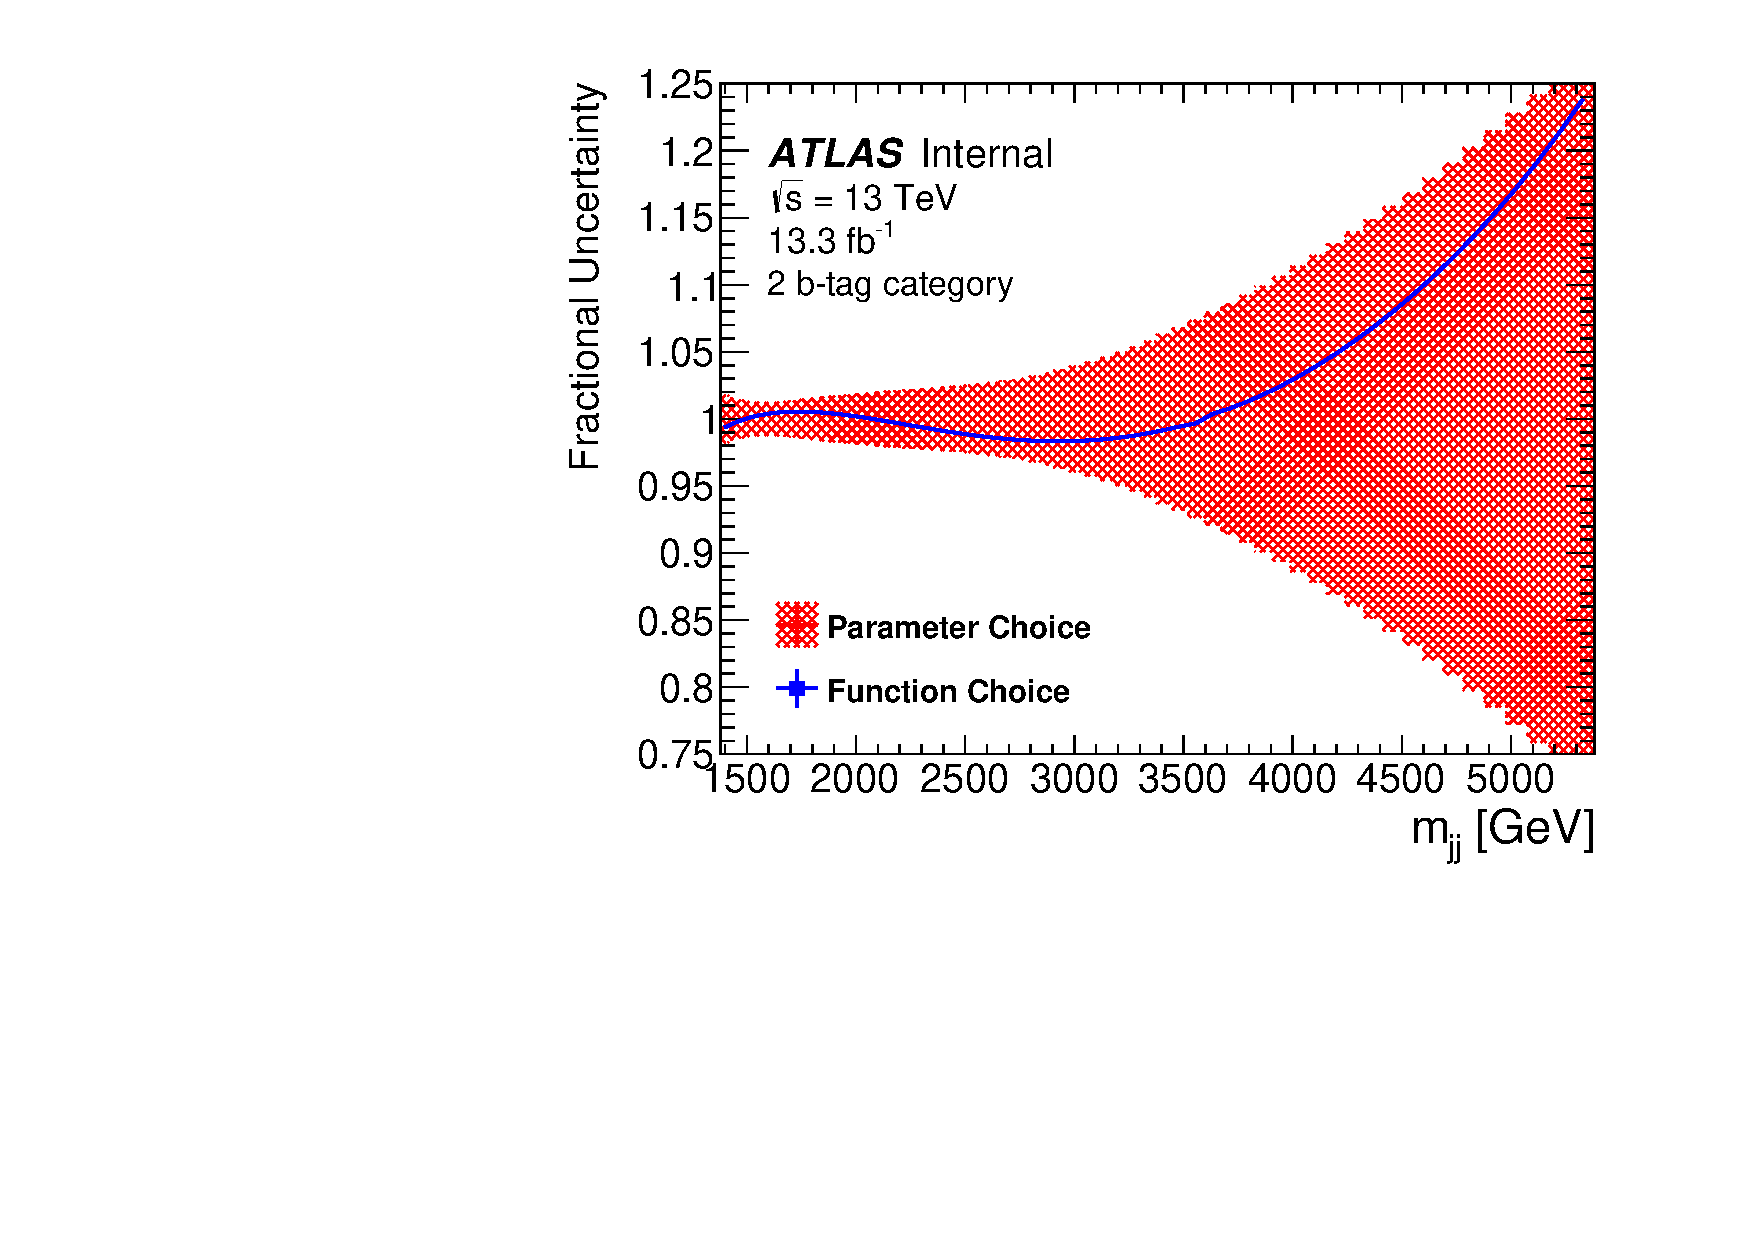
\includegraphics[width=0.47\linewidth, angle=0]{figs/Dibjet/ICHEP/lim-summer_systBkg_bb.pdf}}
    \subcaptionbox{$\geq$1 $b$-tag}{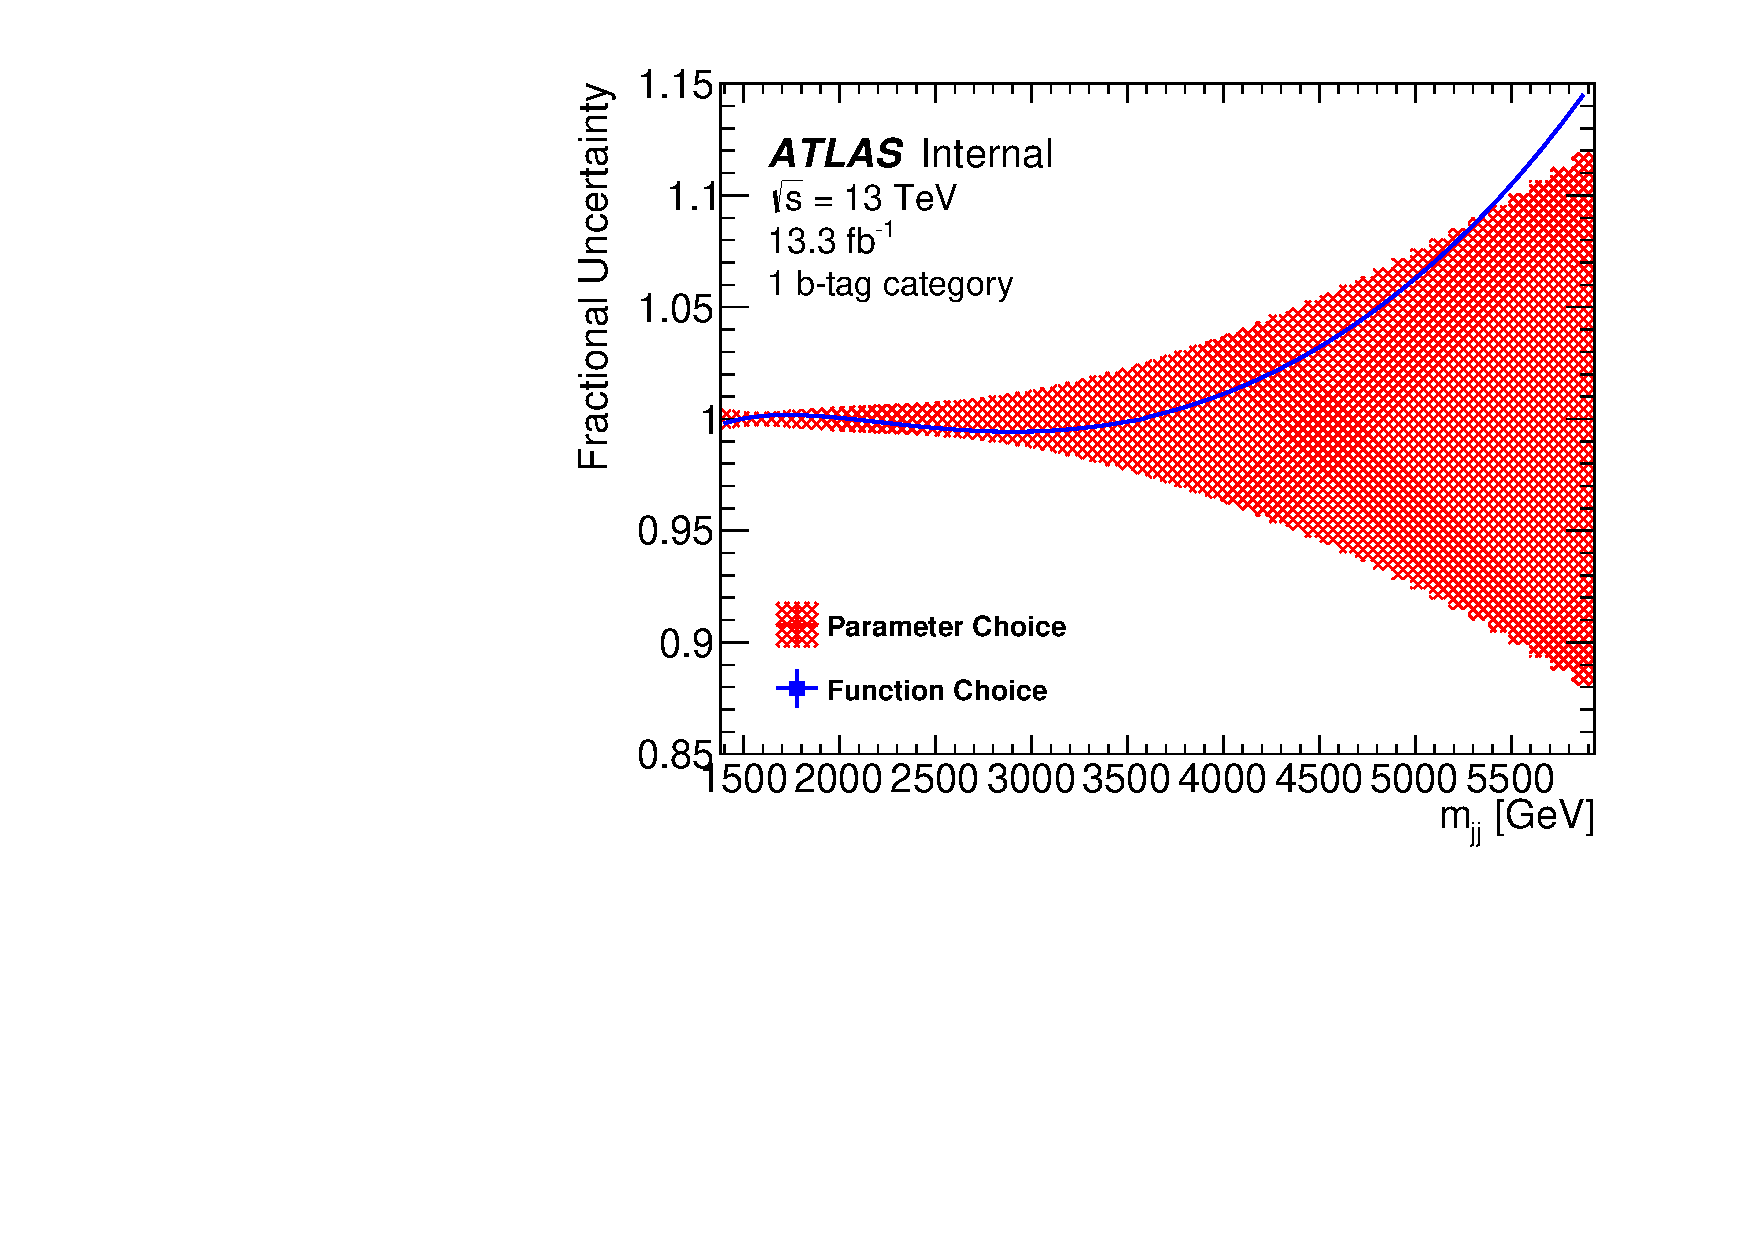
\includegraphics[width=0.47\linewidth, angle=0]{figs/Dibjet/ICHEP/lim-summer_systBkg_b.pdf}}
  \end{center}
  \vspace{-1mm}
  \caption{The background systematic uncertainties for the (a) 2 and (b) $\geq$1 $b$-tag categories
    as a function of dijet mass,~\mjj, for the \textit{Summer16+15} data-set.
    The red shaded region shows the function parameter uncertainty and the
    function choice uncertainty is shown by the blue line. }
  \label{fig:lim-summer_systBkg}
\end{figure}

%Figure~\ref{fig:lim-summer_zprime} and \ref{fig:lim-summer_bstar} show the %% When there was two
Figure~\ref{fig:lim-summer_benchmark} shows the
95\% credibility level upper limits set on $\sigma\,\text{x}\,\mathit{A}\,\text{x}\,\epsilon$
as a function of simulated mass
for the $Z'$-boson and a $b^*$-quark.
%The signal models considered are described in Section~\ref{sec:evt-s+b}.
The observed limit, the expected limit and the 1 and 2 $\sigma$ uncertainty bands on the expected limit are shown.
The $\geq1$ $b$-tag category is used for the $b^*$-quark model
and the 2 $b$-tag category is used for the $Z'$-boson models
as these categories provide the strongest limits on the models.
Overlaid are theoretical predictions of
$\sigma\,\text{x}\,\mathit{A}\,\text{x}\,\epsilon$ for the benchmark models described in Section~\ref{sec:evt-s+b}.

%\begin{figure}[!ht]
%  \centering
%   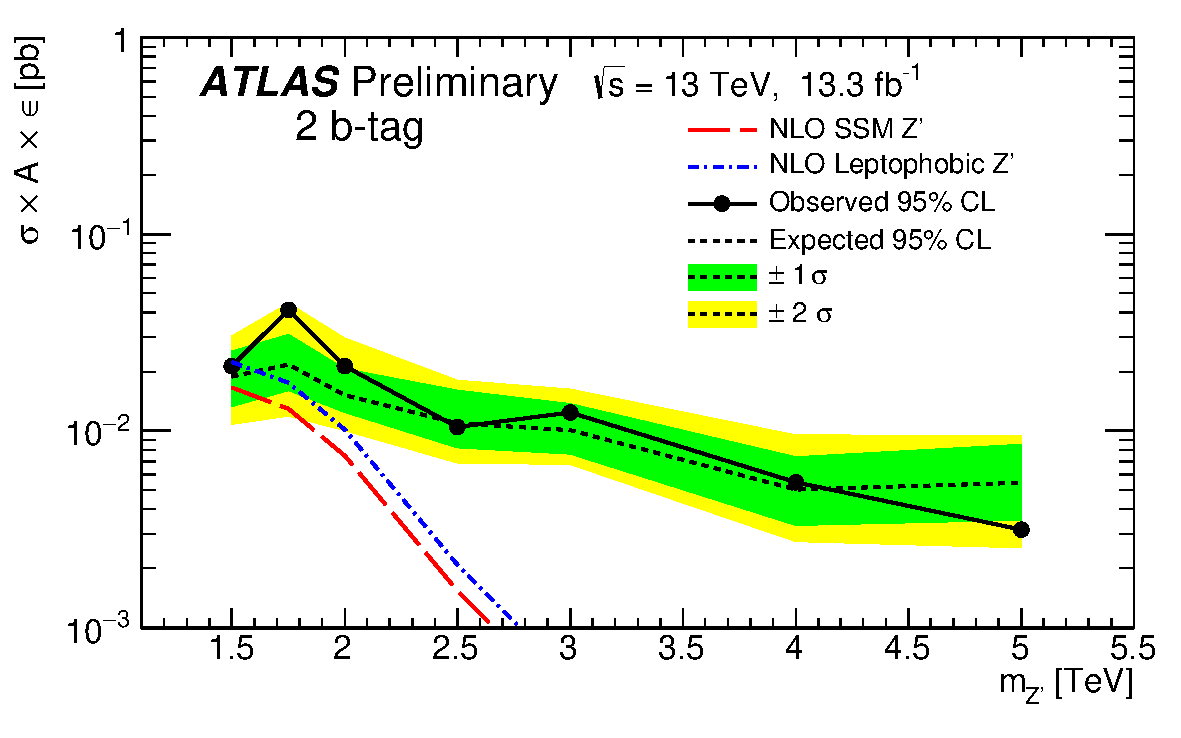
\includegraphics[width=0.7\linewidth, angle=0]{figs/Dibjet/ICHEP/lim-zprime.pdf}
%   \caption[Bayesian 95\% credibility level upper limits on cross-section times acceptance times tagging efficiency
%     for the $Z'$-boson as a function of simulated mass
%     for the 2 $b$-tag category using the \textit{Summer16+15} data-set.
%     The observed limit is shown by the solid black line,
%     the expected limit is shown by the dotted black line
%     and the 1 and 2 $\sigma$ uncertainty bands are shown by the green and yellow bands respectively.
%     The theoretical predicition of $\sigma\,\text{x}\,\mathit{A}\,\text{x}\,\epsilon$
%     for the Sequential Standard Model (SSM) and leptophobic $Z'$-boson are overlaid.]
%           {Bayesian 95\% credibility level upper limits on cross-section times acceptance times tagging efficiency
%             for the $Z'$-boson as a function of simulated mass
%             for the 2 $b$-tag category using the \textit{Summer16+15} data-set.
%             The observed limit is shown by the solid black line,
%             the expected limit is shown by the dotted black line
%             and the 1 and 2 $\sigma$ uncertainty bands are shown by the green and yellow bands respectively.
%             The theoretical predicition of $\sigma\,\text{x}\,\mathit{A}\,\text{x}\,\epsilon$
%             for the Sequential Standard Model (SSM) and leptophobic $Z'$-boson are overlaid~\cite{dibjet-ichep_conf}.
%           }
%  \label{fig:lim-summer_zprime}
%  \vspace{1cm}
%  \centering
%   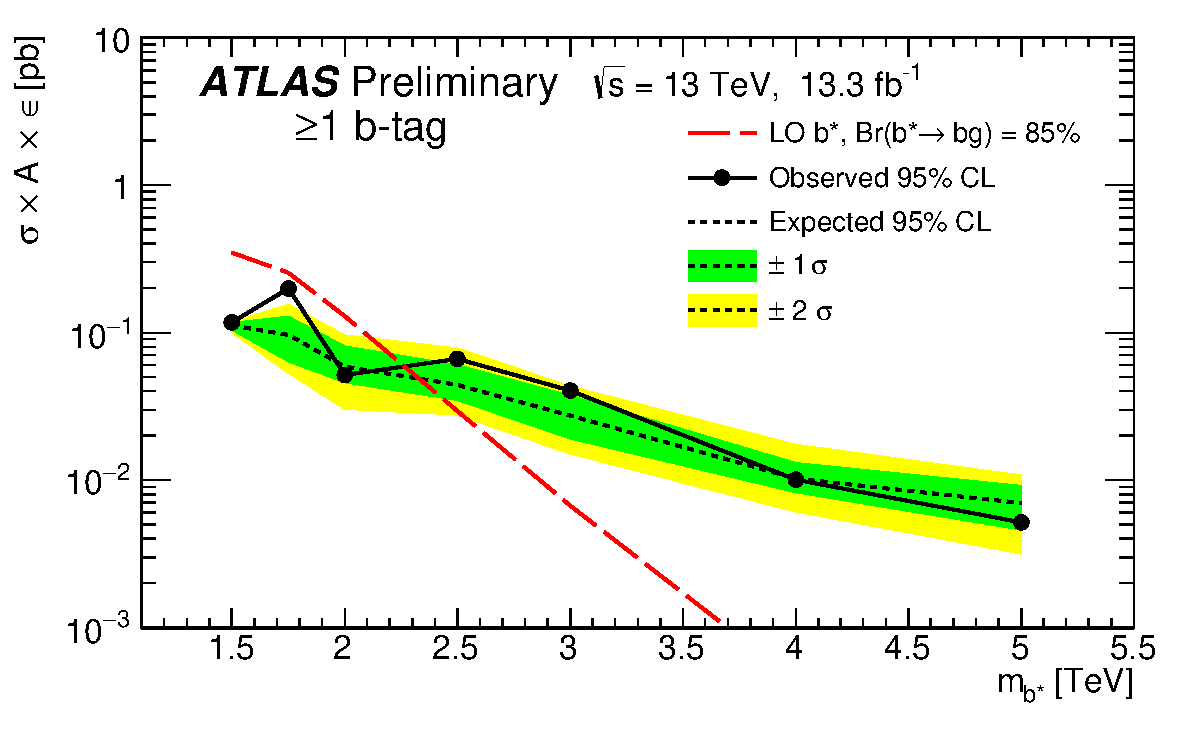
\includegraphics[width=0.7\linewidth, angle=0]{figs/Dibjet/ICHEP/lim-bstar.pdf}
%   \caption[Bayesian 95\% credibility level upper limits on cross-section times acceptance times tagging efficiency
%    for the $b^*$-quark  as a function of simulated mass
%    for the $\geq$1 $b$-tag category using the \textit{Summer16+15} data-set.
%    The observed limit is shown by the solid black line,
%    the expected limit is shown by the dotted black line
%    and the 1 and 2 $\sigma$ uncertainty bands are shown by the green and yellow bands respectively.
%    The theoretical predicition of $\sigma\,\text{x}\,\mathit{A}\,\text{x}\,\epsilon$
%    for the $b^*$-quark is overlaid.]
%           {Bayesian 95\% credibility level upper limits on cross-section times acceptance times tagging efficiency
%             for the $b^*$-quark  as a function of simulated mass
%             for the $\geq$1 $b$-tag category using the \textit{Summer16+15} data-set.
%             The observed limit is shown by the solid black line,
%             the expected limit is shown by the dotted black line
%             and the 1 and 2 $\sigma$ uncertainty bands are shown by the green and yellow bands respectively.
%             The theoretical predicition of $\sigma\,\text{x}\,\mathit{A}\,\text{x}\,\epsilon$
%             for the $b^*$-quark is overlaid~\cite{dibjet-ichep_conf}.
%           }
%  \label{fig:lim-summer_bstar}
%\end{figure}


\begin{figure}[!ht]
  \centering
  \captionsetup[subfigure]{aboveskip=0pt,justification=centering}
  \subcaptionbox{$Z'$-boson,\hspace{1mm} 2 $b$-tag}{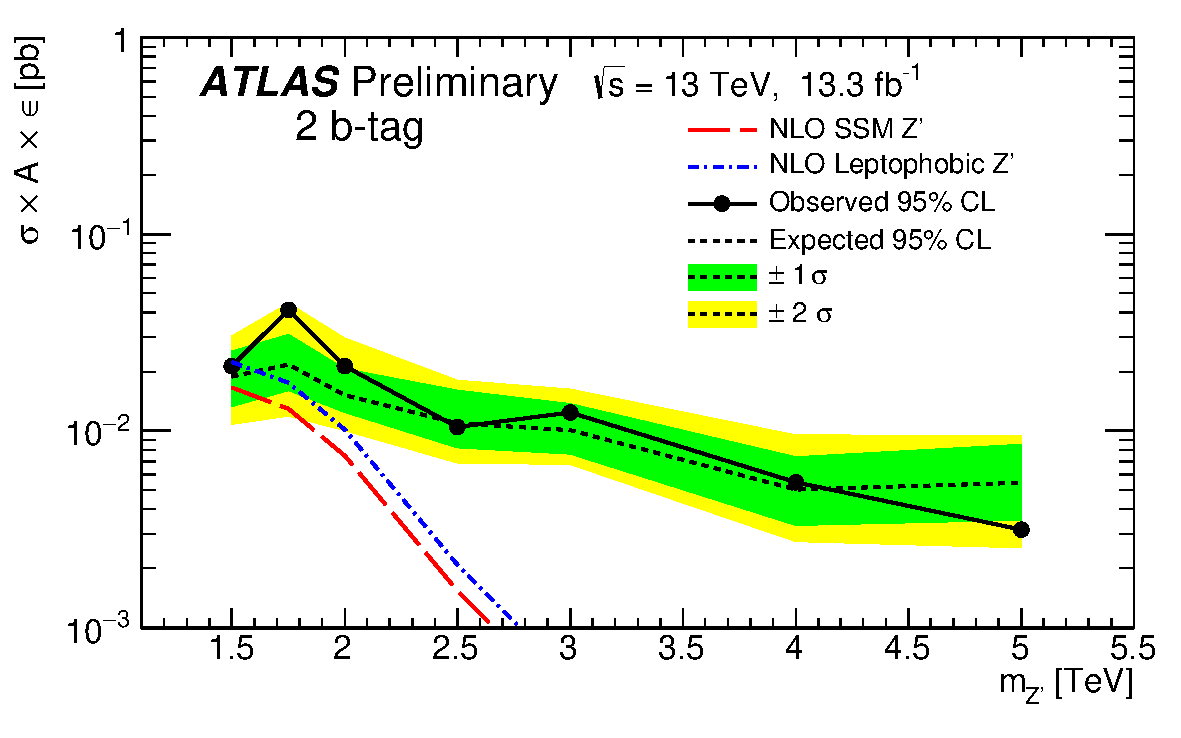
\includegraphics[width=0.8\linewidth, angle=0]{figs/Dibjet/ICHEP/lim-zprime.pdf}}
  \hspace{2mm}
  \subcaptionbox{$b^*$ quark,\hspace{1mm} $\geq$1 $b$-tag}{  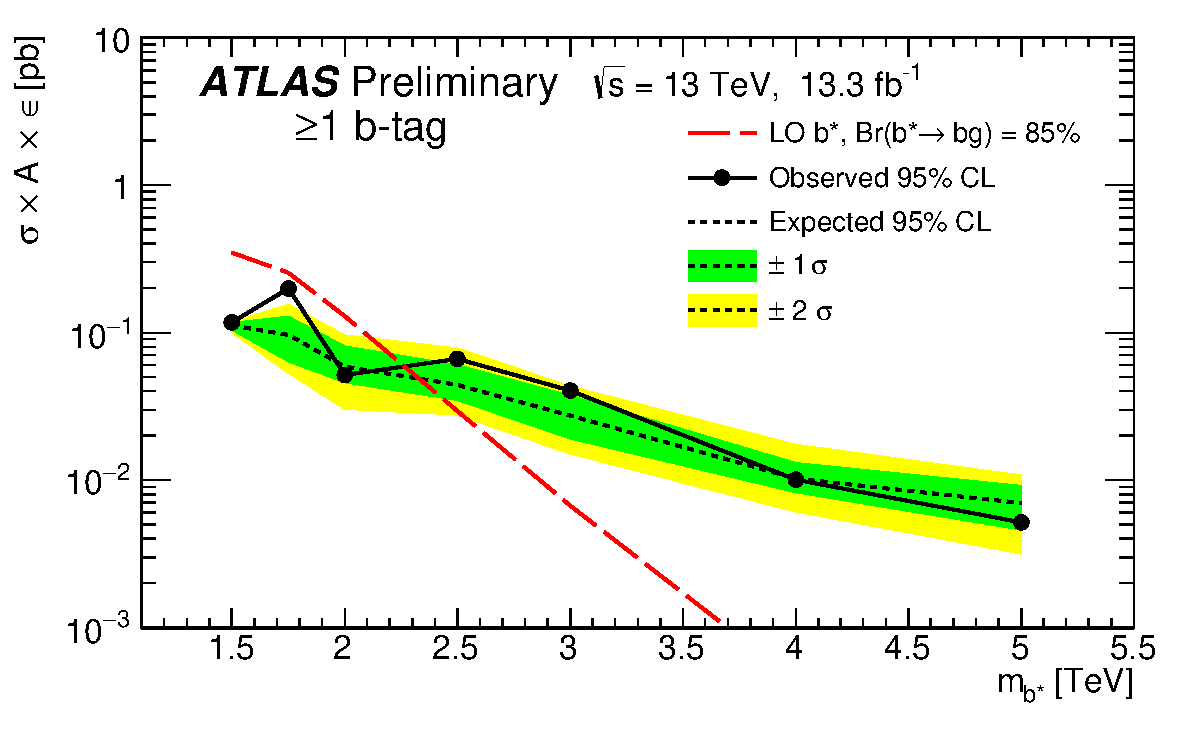
\includegraphics[width=0.8\linewidth, angle=0]{figs/Dibjet/ICHEP/lim-bstar.pdf}}
   \caption[Bayesian 95\% credibility level upper limits on cross-section times acceptance times tagging efficiency
             for the (a) $Z'$-boson and (b) $b^*$-quark  as a function of simulated mass
             using the \textit{Summer16+15} data-set in the 2 and $\geq$1 $b$-tag category respectively.
             The observed limit is shown by the solid black line,
             the expected limit is shown by the dotted black line
             and the 1 and 2 $\sigma$ uncertainty bands on the expected limit are shown by the green and yellow bands.
             The theoretical prediction of $\sigma\,\text{x}\,\mathit{A}\,\text{x}\,\epsilon$
             for the Sequential Standard Model (SSM) and leptophobic $Z'$-boson and the $b^*$-quark are overlaid.]
           {Bayesian 95\% credibility level upper limits on cross-section times acceptance times tagging efficiency
             for the (a) $Z'$-boson and (b) $b^*$-quark  as a function of simulated mass
             using the \textit{Summer16+15} data-set in the 2 and $\geq$1 $b$-tag category respectively.
             The observed limit is shown by the solid black line,
             the expected limit is shown by the dotted black line
             and the 1 and 2 $\sigma$ uncertainty bands on the expected limit are shown by the green and yellow bands.
             The theoretical prediction of $\sigma\,\text{x}\,\mathit{A}\,\text{x}\,\epsilon$
             for the Sequential Standard Model (SSM) and leptophobic $Z'$-boson and the $b^*$-quark are overlaid~\cite{dibjet-ichep_conf}.
           }
  \label{fig:lim-summer_benchmark}
\end{figure}

The observed and expected limits decrease with increasing simulated mass
due to reduced number of background events at higher mass.
The theoretical $\sigma\,\text{x}\,\mathit{A}\,\text{x}\,\epsilon$ predictions
decrease rapidly as mass increases, due to a combination of
lower signal acceptance times efficiency at high mass, as shown in Figures~\ref{fig:evt-ichep_acc},
and a smaller signal cross-section at high mass.
The signal cross-section is smaller at high mass because of PDF and matrix element effects,
similar to those that caused a smaller QCD dijet production at high mass as described in
 Section~\ref{sec:theo-qcd-dijet_features}.

In the mass regions where the theoretical prediction of $\sigma\,\text{x}\,\mathit{A}\,\text{x}\,\epsilon$
is larger than the upper limit, it can be concluded that the model is excluded at the 95\% credibility level.
Using the \summer{} data-set:
the \mbox{$b^*$-quark} is excluded in the mass range of 1.38 - 2.3 TeV,
the SSM $Z'$-boson cannot be excluded,
and the leptophobic $Z'$-boson is excluded at a mass of 1.5 TeV.

To produce generic Gaussian limits ,
a signal template with a Gaussian shape in dijet mass is used.
The Gaussian shapes are centred on a range of masses
and the width of the considered Gaussians are
15\%, 10\%, 7\% of the simulated mass
in addition to a Gaussian with the width of the detector mass resolution.
The detector mass resolution has been estimated
at previous dijet searches~\cite{dijet-mori16_paper}
and varies from 3\% at 1.5 TeV to 2\% at 5 TeV.
%The dijet mass resolution is defined as the width of a Gaussian fit to mreco/mtruth
% for matched leading and subleading jets divided by the mean of the Gaussian.
For the Gaussian limits the sources of the systematic uncertainty considered
are the luminosity uncertainty,
the background modelling uncertainties,
and a 10\% flat uncertainty to account sources for
experimental uncertainties related to signal modelling,
such as jet-energy scale.

Figure~\ref{fig:lim-summer_gauss} shows the observed 95\% credibility upper limits
on the product of cross-section, detector acceptance, tagging efficiency and branching ratio,
$\sigma\,\text{x}\,\mathit{A}\,\text{x}\,\epsilon\,\text{x}\,\mathit{BR}$,
for the full range of Gaussian signals described above in both $b$-tagging categories.
For the \summer{} an upper limit is placed on a generic Gaussian signal
ranging from 0.2 to 0.001 pb is set in the mass range 1.4 to 6 TeV.

\begin{figure}[!ht]
  \begin{center}
    \captionsetup[subfigure]{aboveskip=0pt,justification=centering}
   \subcaptionbox{2 $b$-tag}      {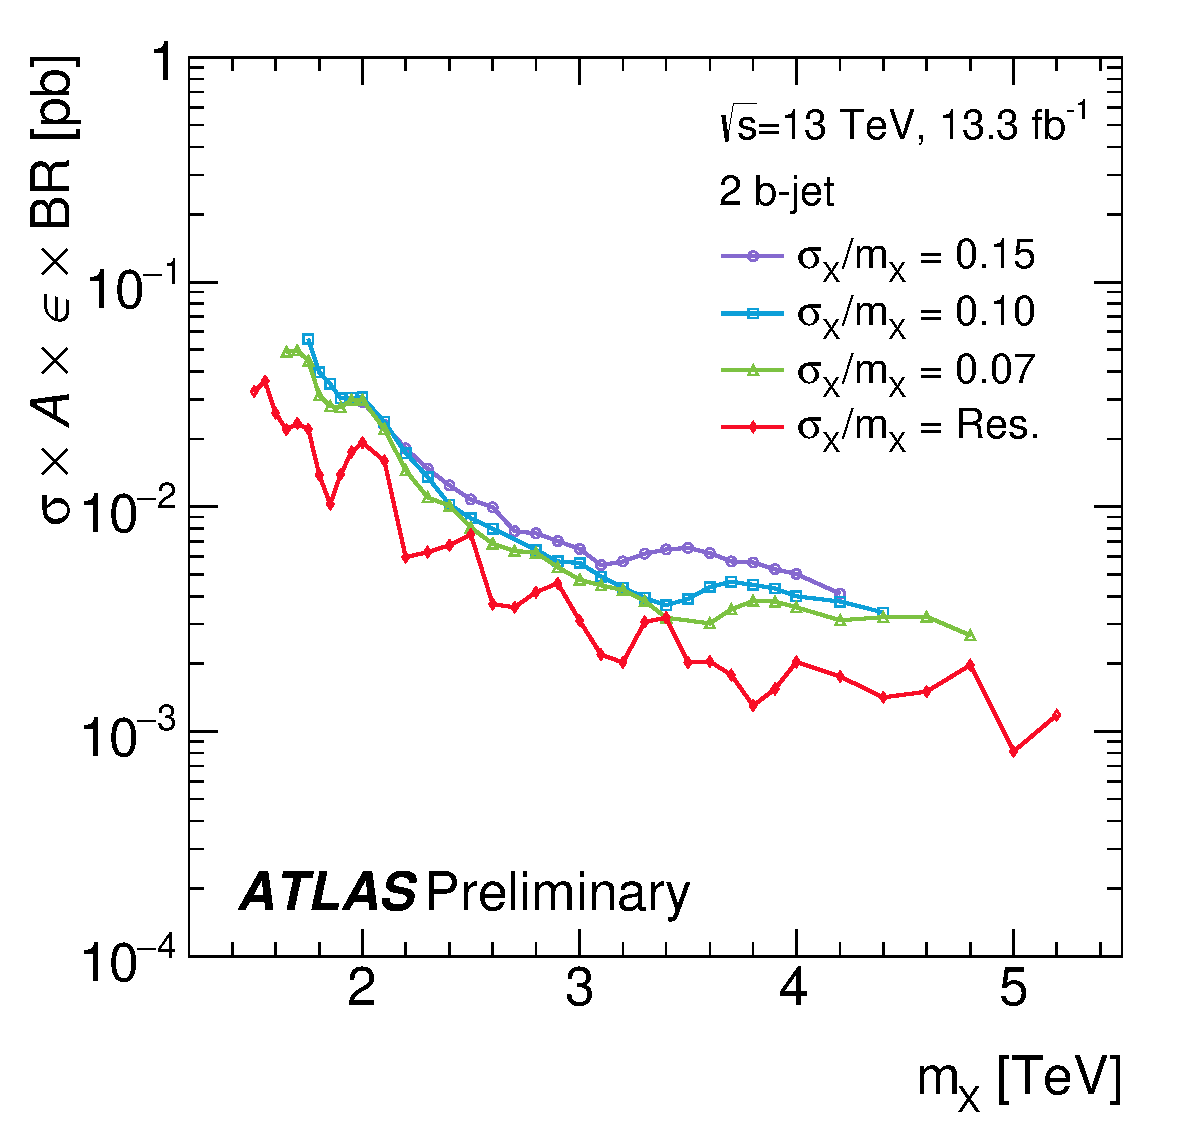
\includegraphics[width=0.47\linewidth, angle=0]{figs/Dibjet/ICHEP/lim-summer_gauss_bb.pdf}}
   \subcaptionbox{$\geq$1 $b$-tag}{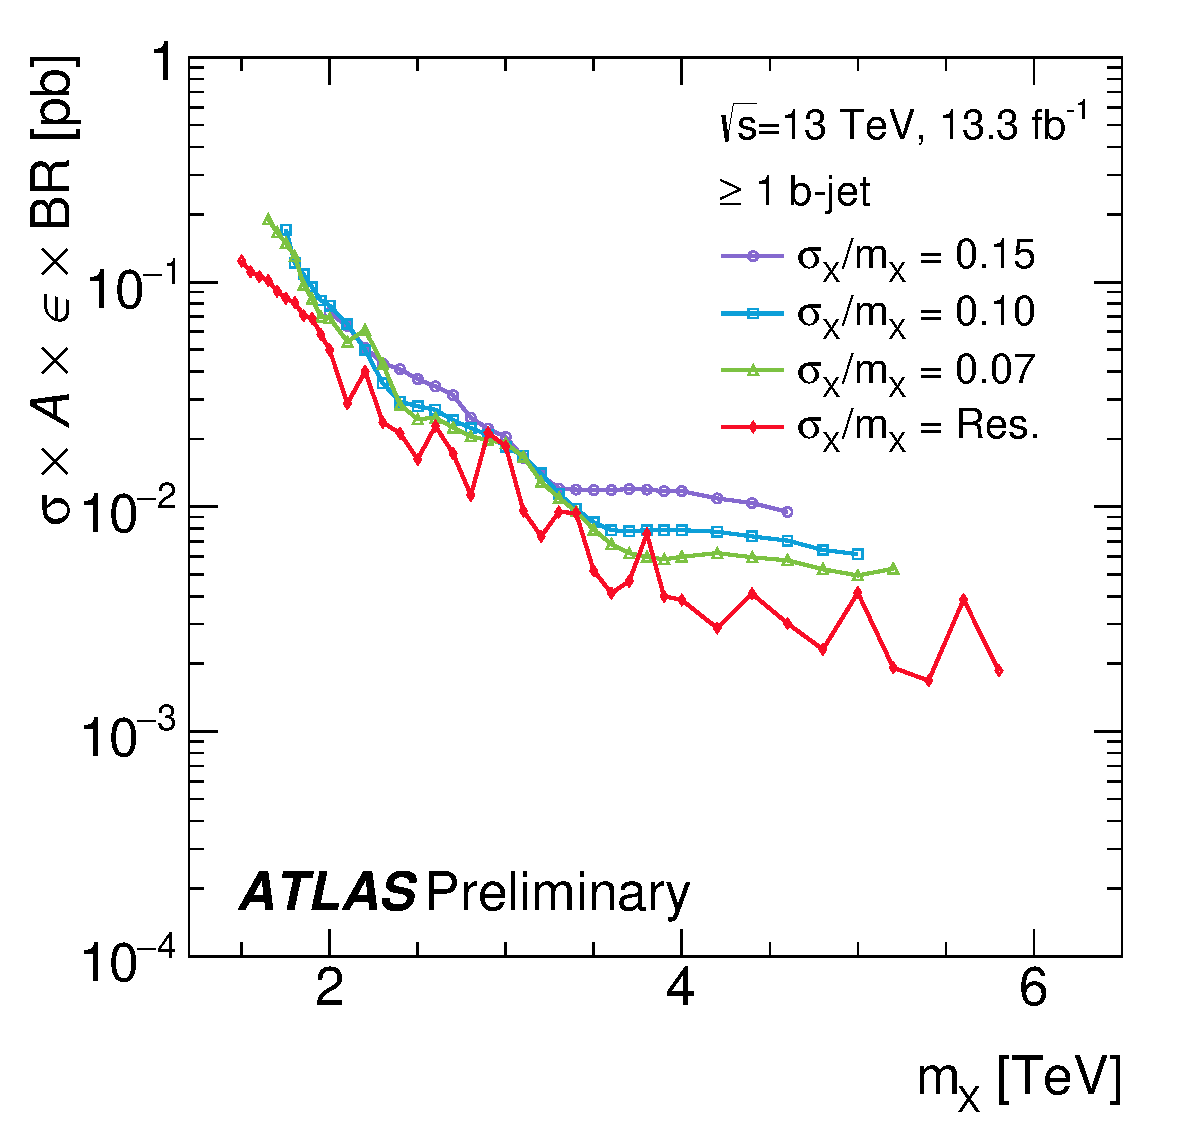
\includegraphics[width=0.47\linewidth, angle=0]{figs/Dibjet/ICHEP/lim-summer_gauss_b.pdf}}
  \end{center}
  \caption[95\% credibility observed upper limits
    on the product of cross-section, detector acceptance, tagging efficiency and branching ratio,
    $\sigma\,\text{x}\,\mathit{A}\,\text{x}\,\epsilon\,\text{x}\,\mathit{BR}$,
    for Gaussian signals for both $b$-tagging categories using the \textit{Summer16+15} data-set.
    The Gaussian widths considered are 15\%, 10\% and 7\% of the simulated mass
    in addition to a Gaussian with the width of the detector mass resolution.]
  {95\% credibility observed upper limits
    on the product of cross-section, detector acceptance, tagging efficiency and branching ratio,
    $\sigma\,\text{x}\,\mathit{A}\,\text{x}\,\epsilon\,\text{x}\,\mathit{BR}$,
    for Gaussian signals for both $b$-tagging categories using the \textit{Summer16+15} data-set.
    The signal templates are Gaussian in dijet  mass with
    widths of 15\%, 10\% and 7\% of the simulated mass
    in addition to a Gaussian with the width of the detector mass resolution~\cite{dibjet-ichep_conf}.
  }
  \label{fig:lim-summer_gauss}
\end{figure}

\FloatBarrier

\section{\lm{} Data-set Limits}
\label{sec:lim-full}

\subsection{Signal Morphing}
\label{sec:lim-full_morphing}

The limit setting procedure requires dijet mass signal templates as an input.
For the \lm{} data-set analysis, simulated dijet mass signal templates of the SSM $Z'$ boson are created at simulated mass points of
600, 800, 1000 and 1250 GeV, as described in Section~\ref{sec:evt-s+b}.
To obtain dijet mass signal templates for intermediate points a signal morphing technique is used,
first implemented in an inclusive ATLAS dijet search~\cite{dijet-mori17_paper}.

A `Gaussian + reverse Landau' fit is performed to the simulated dijet mass signal templates.
The reverse Landau function is the transformation of the Landau function~\cite{lim-landau} under $x\to-x$.
The Gaussian + reverse Landau fit function is therefore defined as:
\begin{equation}
  f(x)=p_0 \left[ \,p_3\,\mathrm{Gauss}\left(x,p_1,p_2\right)\,+\,\left(\,1-p_3\,\right)\,\mathrm{Landau}\,\left(-x,p_4,p_5\right)\, \right]
\end{equation}
The Gaussian distribution models the convolution of a Breit-Wigner resonance distribution and mass resolution effects.
The reverse Landau distribution provides a description of the off-shell contributions to the dijet mass signal templates which are enhanced at low mass by PDF effects.

The parameters of the Gaussian + reverse Landau fits are interpolated to produce dijet mass signal templates at intermediary simulated mass points
in the range 600 to 1250 GeV with a separation of 50 GeV
\footnote{Explicitly morphed signal templates are created at simulated mass points of
  650, 700, 750, 850, 900, 950, 1050, 1100, 1150 and 1200 GeV.}.
Figure~\ref{fig:lim-full_morphing} shows the simulated SSM $Z'$ boson dijet mass signal templates and the intermediate dijet mass signal templates produced using the morphing procedure.
The simulated and morphed signal dijet mass spectra are used as signal templates in the limit setting procedure for the \lm{} data-set analysis.
  
\begin{figure}[!ht]
\begin{center}
  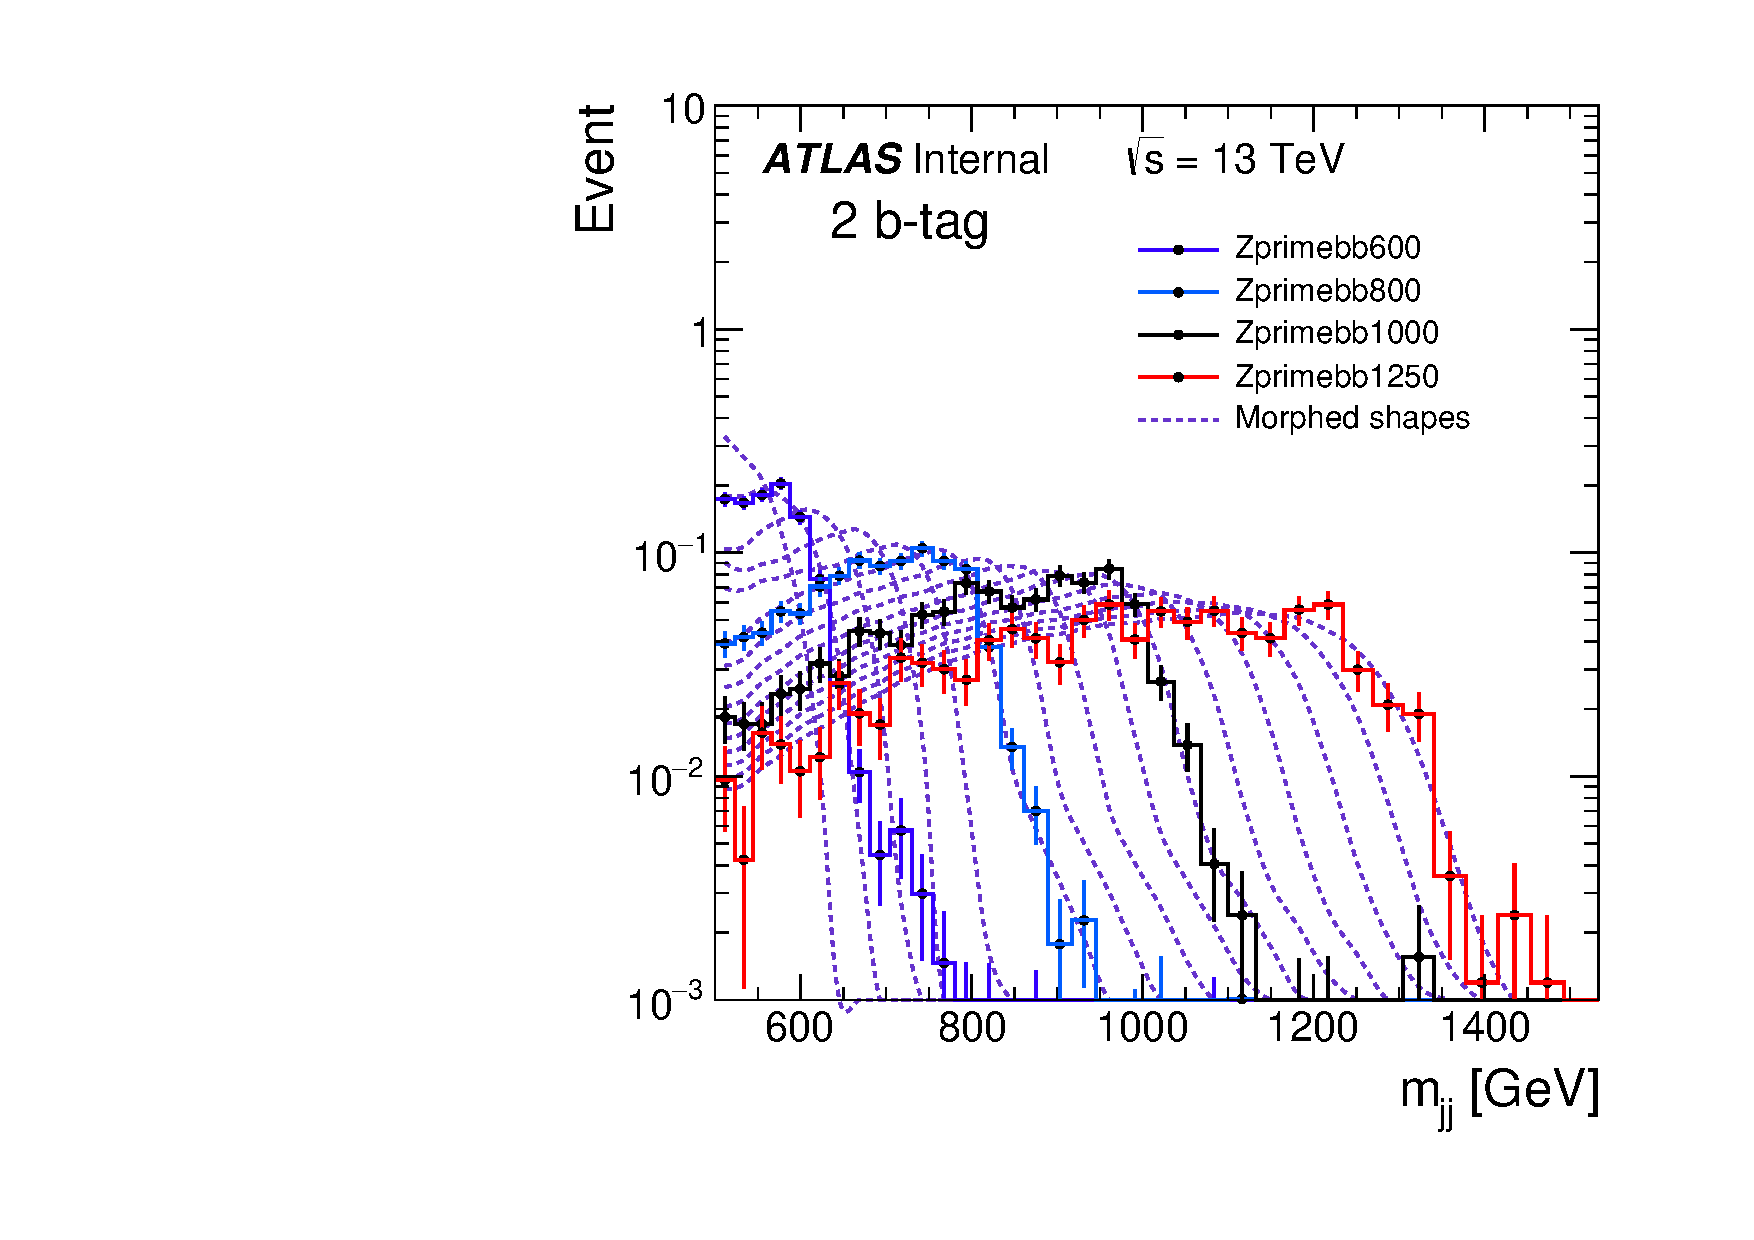
\includegraphics[width=0.5\linewidth, angle=0]{figs/Dibjet/LowMass/lim-morphing.pdf} 
\end{center}
\caption[Simulated SSM $Z'$ boson dijet mass (\mjj) signal templates and the intermediate dijet mass signal templates
  created using the signal morphing technique used in the \lm{} data-set limit setting phase.]
        {Simulated SSM $Z'$ boson dijet mass (\mjj) signal templates (solid points lines)
          at simulated mass points of 600, 800, 1000 and 1250 GeV 
          and the dijet mass signal templates created using the signal morphing technique (dotted lines) used in the \lm{} data-set limit setting phase~\cite{dibjet-full_int}.
          \label{fig:lim-full_morphing}}
\end{figure}




\subsection{Summary of Systematic Uncertainties}
\label{sec:lim-full_systs}

Table~\ref{tab:lim-lowmass_syst} summarises the systematic uncertainties considered for the
signal templates used in the \lm{} data-set at three different dijet masses (\mjj{}).
Figure~\ref{fig:lim-lowmass_syst}(a) shows the total $b$-jet trigger systematic uncertainty as a function of dijet  mass;
this includes both the jet-level and event-level uncertainties described in Section~\ref{sec:trig-bjet_eff}.
Figure~\ref{fig:lim-lowmass_syst}(b) shows the systematic uncertainties on the background estimate as a function of dijet  mass.
%Reconstructed mass is defined as invariant mass of the two observed jets.
%$b$-tagging, $b$-jet trigger and $b$-jet energy scale are the dominant sources of systematic uncertainties at the lowest mass point,
%whilst for the remaining dijet mass range $b$-jet trigger uncertainties are dominant.

\begin{table}[!htb]
  \centering
  \begin{tabular}{|c||c|c|c|c|c|c|c|}
    \hline
    \mjj    & \multicolumn{7}{c|}{Signal Systematic Uncertainties}                    \\ \cline{2-8} 
            & JES   & JER   & $b$JES  & $b$-Tagging & $b$-Jet Trigger & PDF & Lumi        \\
    \hline                                                                        
    0.5 TeV & 0.9\% & 1.4\% & 5\%     &     5\%     &      5.4\%   & 1\% & 2.2\%       \\
    1.0 TeV & 0.8\% & 1.2\% & 3\%     &     7\%     &       15\%   & 1\% & 2.2\%       \\
    1.5 TeV & 1.1\% & 1.0\% & 1.8\%    &    10\%     &       29\%   & 1\% & 2.2\%       \\
    \hline
    % The background uncertainties
    %& \multicolumn{2}{c|}{Bkg. Uncert}             
    %&  Para. ($\geq$1 / 2)   & Func. ($\geq$1 / 2) 
    %                                               
    %&  1.3\%/0.0\%      & 0.3\%/0.0\%              
    %&  3.9\%/1.7\%      & 1.3\%/0.6\%           
    %&   22\%/ 17\%      & 7.5\%/5.1\%
  \end{tabular}
  \caption[A table summarising the signal systematic uncertainties used in the \lm{} data-set.]
          {A table summarising the signal systematic uncertainties used in the \lm{} data-set
           for three different dijet mass (\mjj{}) points .
          Jet Energy Scale (JES), Jet Energy Resolution (JER) and $b$-jet Energy Scale ($b$JES)
          are uncertainties on the dijet mass of a simulated event,
          whilst $b$-tagging, $b$-jet trigger, PDF and luminosity uncertainties are uncertainties on simulated event weight.
          Values taken from~\cite{dibjet-full_int}}
  \label{tab:lim-lowmass_syst}
  \end{table}

\begin{figure}[!ht]
  \begin{center}
    \captionsetup[subfigure]{aboveskip=0pt,justification=centering}
    \subcaptionbox{$b$-Jet Trigger Uncertainty}{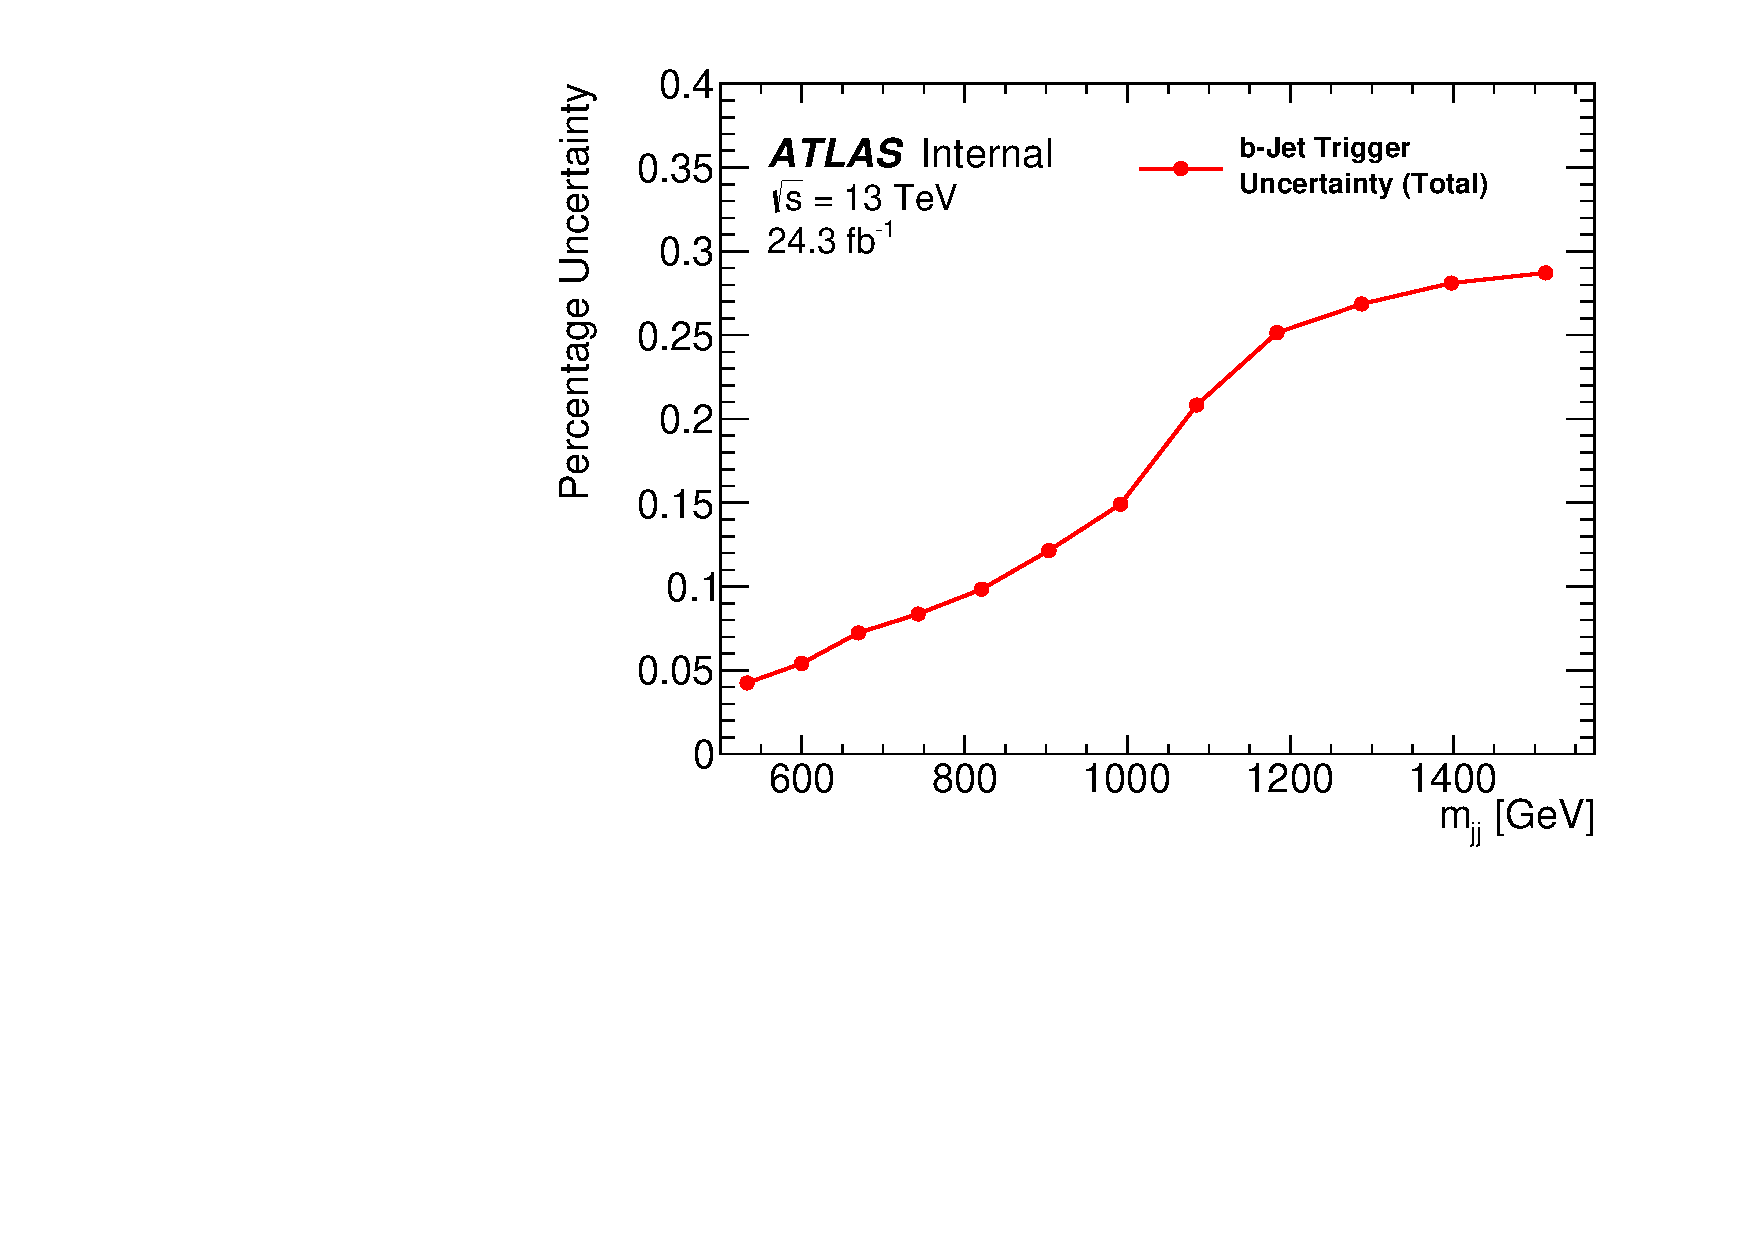
\includegraphics[width=0.47\linewidth, angle=0]{figs/Dibjet/LowMass/lim-bTrigUncert.pdf}}
    \subcaptionbox{Background Uncertainties}{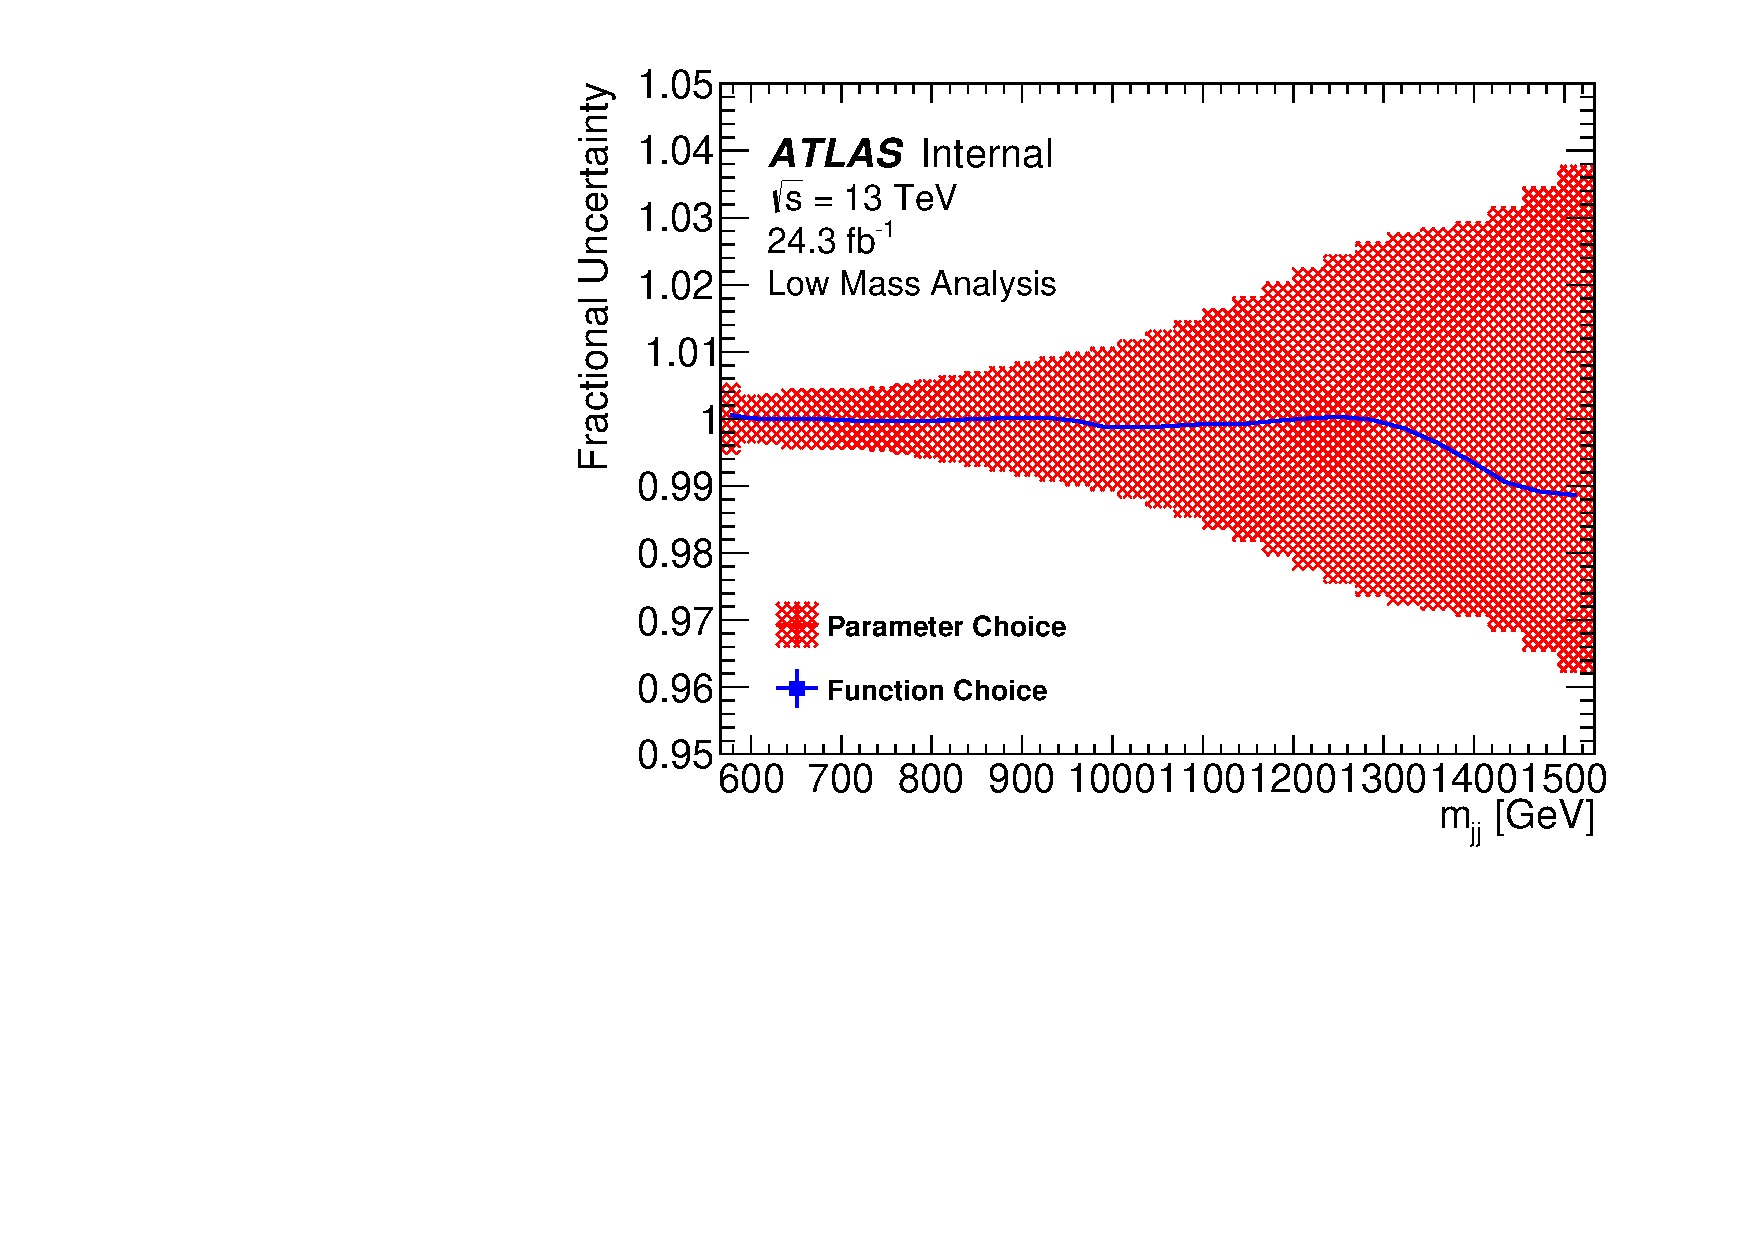
\includegraphics[width=0.47\linewidth, angle=0]{figs/Dibjet/LowMass/lim-lowmass_systBkg.pdf}}
  \end{center}
  \vspace{-1mm}
  \caption{Panel (a) shows the total $b$-jet trigger systematic uncertainty for the \lm{} data-set as a function of dijet mass,~\mjj.
    Panel (b) shows the background systematic uncertainties as a fraction for the \lm{} data-set as a function of dijet mass,~\mjj.
    The red shaded region shows the function parameter uncertainty and the function choice uncertainty is shown by the blue line.}
  \label{fig:lim-lowmass_syst}
\end{figure}

\subsection{Signal Subtracted Background Estimation}
\label{sec:lim-full_ssb}

Section~\ref{sec:bkg-full_swift} described the SWiFt background estimation procedure used for the \lm{} data-set,
for clarity this estimation will be referred to as the nominal SWiFt background estimation in this section.
The nominal SWiFt background estimation is model independent meaning that there is no assumption of any signal models when performing the fit.
In Section~\ref{sec:bkg-full_signalInj} it was found that there is a signal induced fit bias present when
the nominal SWiFt background estimation is performed on a background-only test data-set with a SSM $Z'$ boson injected.
This was particularly notable for a SSM $Z'$ boson with a simulated mass of 600 GeV,
as this is near the edge of the dijet mass spectrum considered.

To remove any signal induced fit bias in the limit setting phase a Signal Subtracted Background (SSB) estimation is
created for each simulated mass point considered, this technique has been used in a previous dijet search at ATLAS~\cite{dijet-mori17_paper}.
The signal subtracted background estimate is created by performing two fits;
the first is a signal plus background fit, performed in the SWiFt window
in which the simulated signal mass being considered is at the window centre.
The signal is modelled using the dijet mass signal templates described in Section~\ref{sec:lim-full_morphing}
and the background is modelled using the 5 parameter dijet fit function.
The normalisation of signal template and the parameters of the background function are
chosen to maximise the likelihood (defined in~\ref{eqn:lim-like}),
the signal normalisation is required to be greater or equal to zero.
The signal template, normalised by the signal plus background fit, is then subtracted from the data.
Finally, the SWiFt background estimation procedure is performed to the signal subtracted data using the 
5 parameter dijet fit function and a window half-width of 16, the same SWiFt configuration used in the search phase results shown in Section~\ref{sec:bkg-full_results}.
This second background estimation is called the signal subtracted background estimation and is used as the background template in the limit setting phase.
A signal subtracted background estimation is created for each signal mass point.

To demonstrate that the signal subtracted background estimation will remove the signal induced fit bias,
fits are performed to a data-like dijet mass spectrum from the fitting control region when SSM $Z'$ boson dijet mass signal templates are injected.
The same distributions were used in the signal injection tests presented in Section~\ref{sec:bkg-full_signalInj}.
The performance of the signal subtracted background estimation can be compared to that of the nominal SWiFt background estimation.

In Figure~\ref{fig:lim-lowmass_ssb_test}(a) the signal subtracted background~(blue) and SWiFt background~(red) estimations
for a data-like dijet mass spectrum from the fitting control region with a SSM $Z'$ boson injected at 600 GeV are
shown as a ratio to the nominal SWiFt background estimation for the same data-like dijet mass spectrum when no signal is injected (black).
This ratio is used to clearly show any fit biases caused by the injected signal.
The signal injected dijet mass spectrum is shown by the green points and the the grey area represents the the statistical uncertainty of the data.
Figure~\ref{fig:lim-lowmass_ssb_test}(b) shows the same comparison using a SSM $Z'$ boson injected at 1000 GeV.
These two mass points are tested as the signal injection tests presented in Section~\ref{sec:bkg-full_signalInj} showed that the search phase
would not produce a significant observation of a SSM $Z'$ boson at these mass points. 

\begin{figure}[!ht]
  \begin{center}
    \captionsetup[subfigure]{aboveskip=0pt,justification=centering}
    \subcaptionbox{$Z'$-boson, $m$ = 600 GeV}{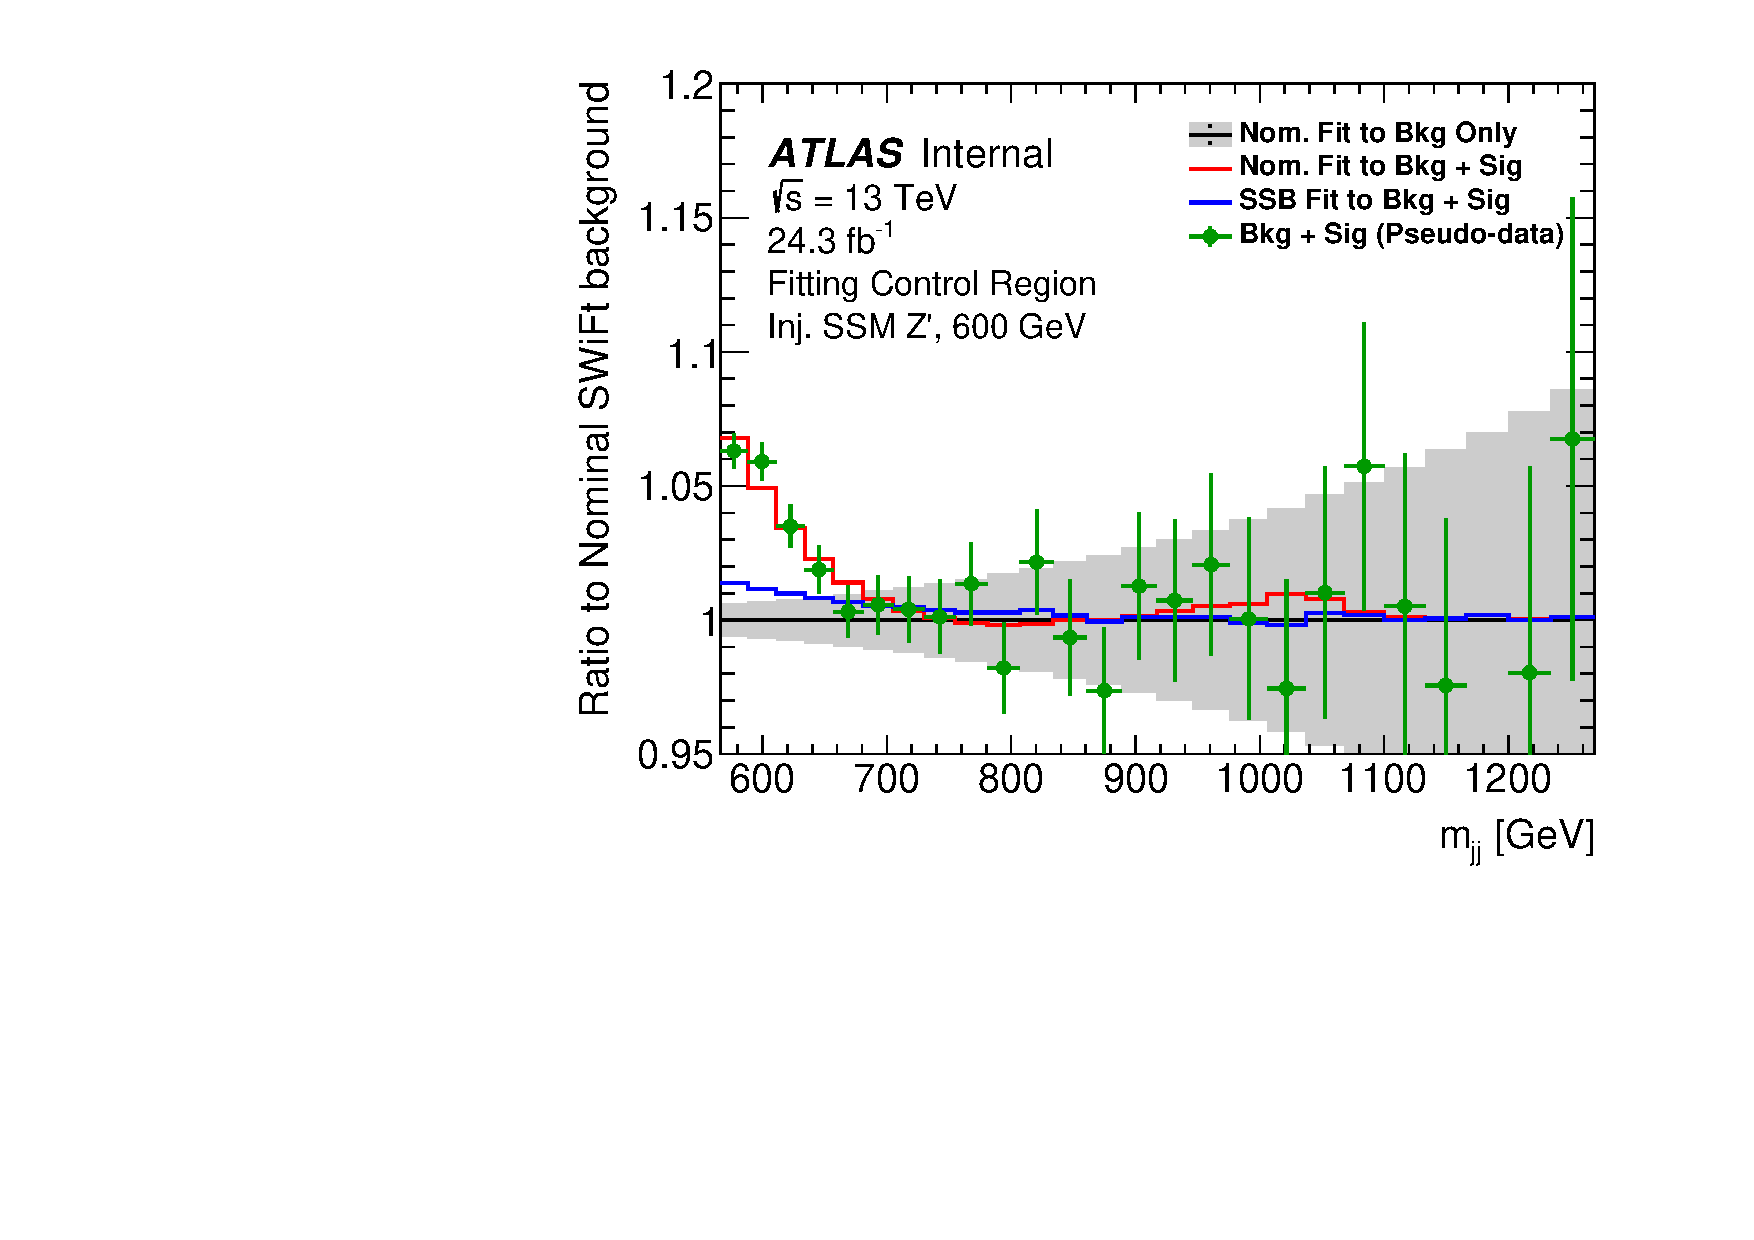
\includegraphics[width=0.47\linewidth, angle=0]{figs/Dibjet/LowMass/lim-ssb_test600.pdf}}
    \subcaptionbox{$Z'$-boson, $m$ = 1000 GeV}{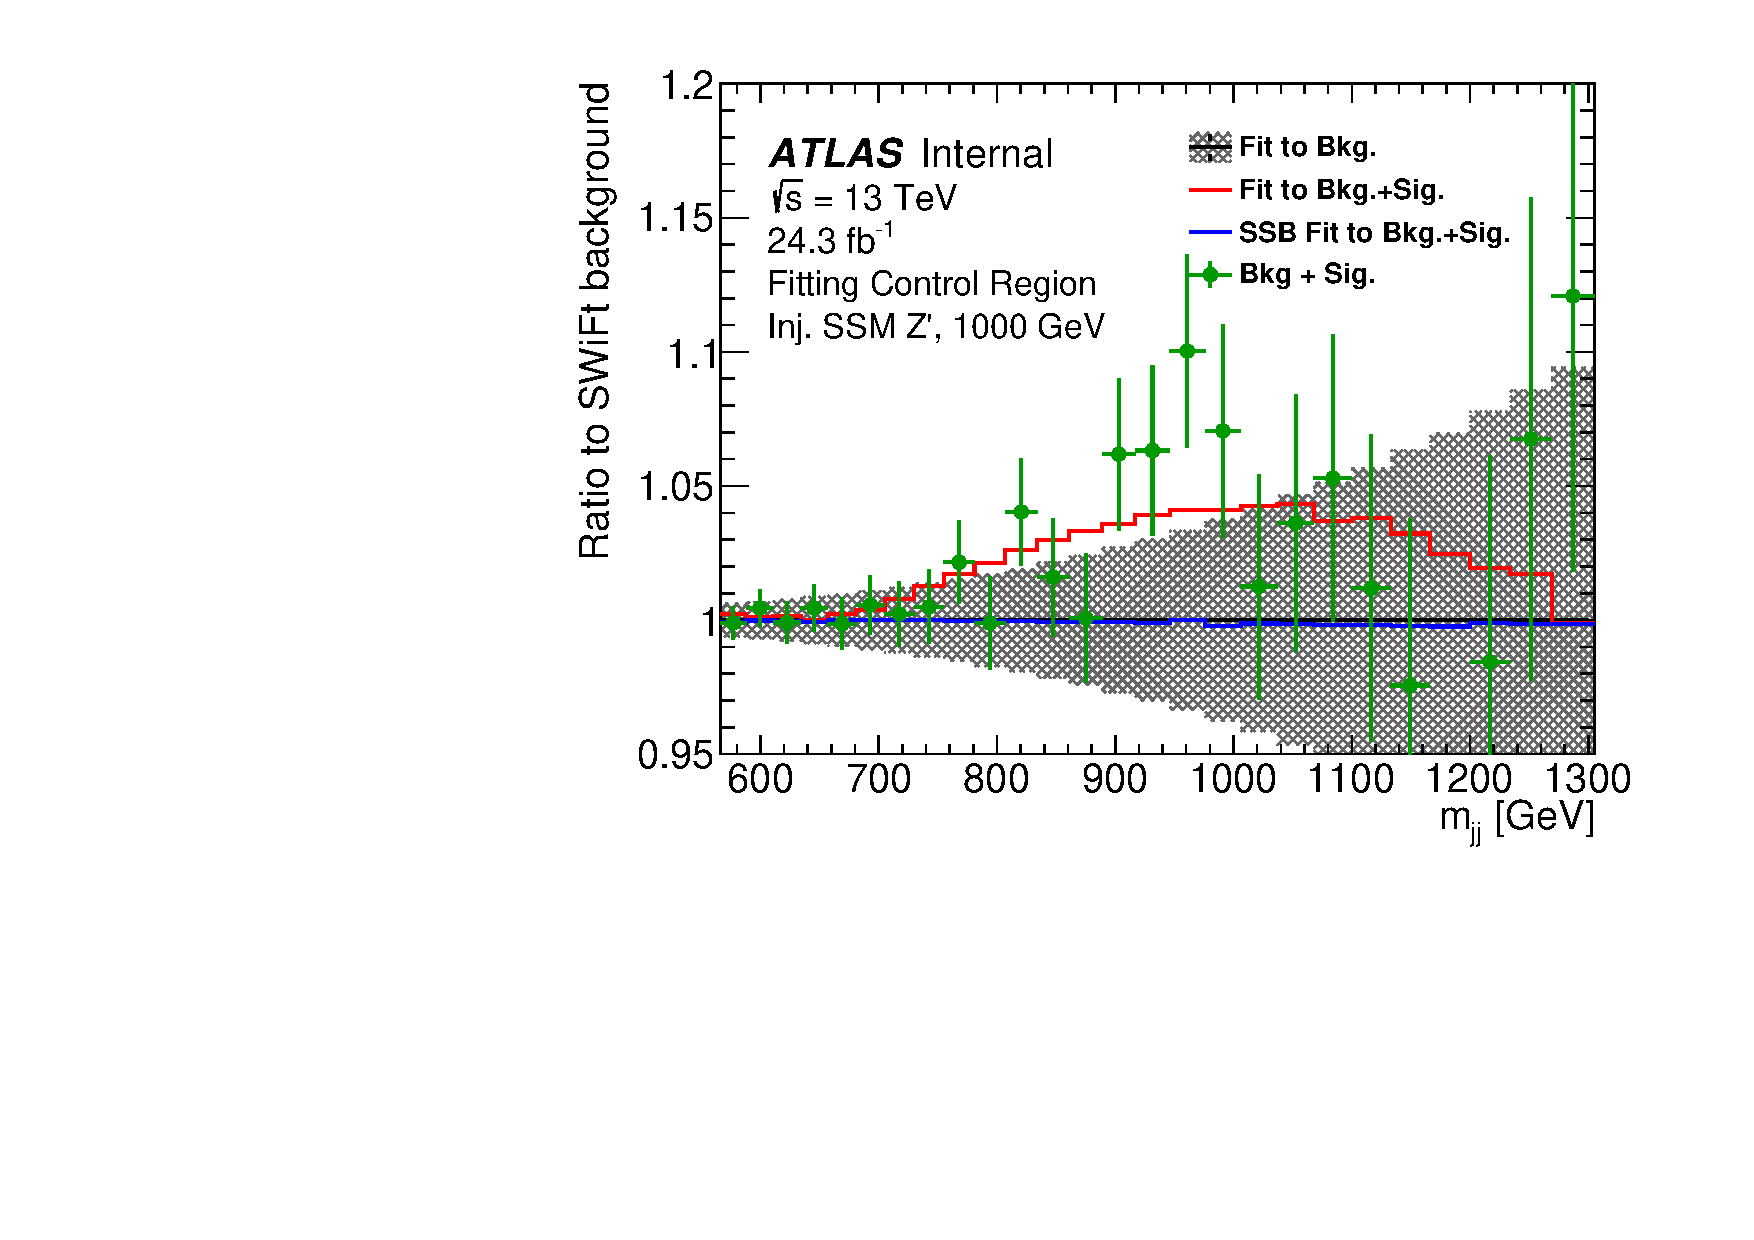
\includegraphics[width=0.47\linewidth, angle=0]{figs/Dibjet/LowMass/lim-ssb_test1000.pdf}}
  \end{center}
  \vspace{-1mm}
  \caption{The nominal background-only SWiFt background (red) and signal subtracted background (SSB) (blue) estimations
    for a data-like dijet mass (\mjj) spectrum from the fitting control region with a SSM $Z'$ boson injected (green points)
    as a ratio to the nominal SWiFt background estimation performed on the same data-like dijet mass spectrum when no signal is applied.
    The area represents the statistical uncertainties in the data-set.
    The simulated mass of the SSM $Z'$ boson is (a) 600 GeV and (b) 1000 GeV.}
  \label{fig:lim-lowmass_ssb_test}
\end{figure}

The nominal SWiFt background estimation is biased when a SSM $Z'$ boson is injected,
shown by the fact that the red line is significantly drawn towards the injected signal in Figure~\ref{fig:lim-lowmass_ssb_test}.
The signal induced fit bias is approximately the same size of the injected signal in the case of a SSM $Z'$ boson at 600 GeV.
It is also observed that the fit bias of the signal subtracted background is small relative to the size of the injected signal.
Therefore, the signal subtracted background is background estimation used in the limit setting phase.

Figure~\ref{fig:lim-lowmass_ssb_data} shows the ratio of the 
signal subtracted background (SSB) estimations and the nominal SWiFt background estimate (black) performed on the full \lm{} data-set
\footnote{The SWiFt background estimate for the full data-set is shown in comparison to the data in Figure~\ref{fig:bhFit_lm_unblind}.}.
The area represents the parameter choice uncertainty of the nominal SWiFt background estimation.
Signal subtracted background estimations are created for all simulated mass points considered,
but for clarity only those at mass points 600, 800, 1000 and 1250 GeV are shown in the figure.
For all simulated mass points, including those not shown in the figure,
the signal subtracted background estimate is consistent with the nominal SWiFt background estimation
within background uncertainties.
Therefore the results of the limit setting phase would be consistent if either the
signal subtracted or nominal SWiFt background estimation are used.
Furthermore, it can be inferred that there is no signal induced fit bias due to a $Z'$ boson
in the nominal SWiFt background estimation performed to the \lm{} data-set.

\begin{figure}[!ht]
  \begin{center}
    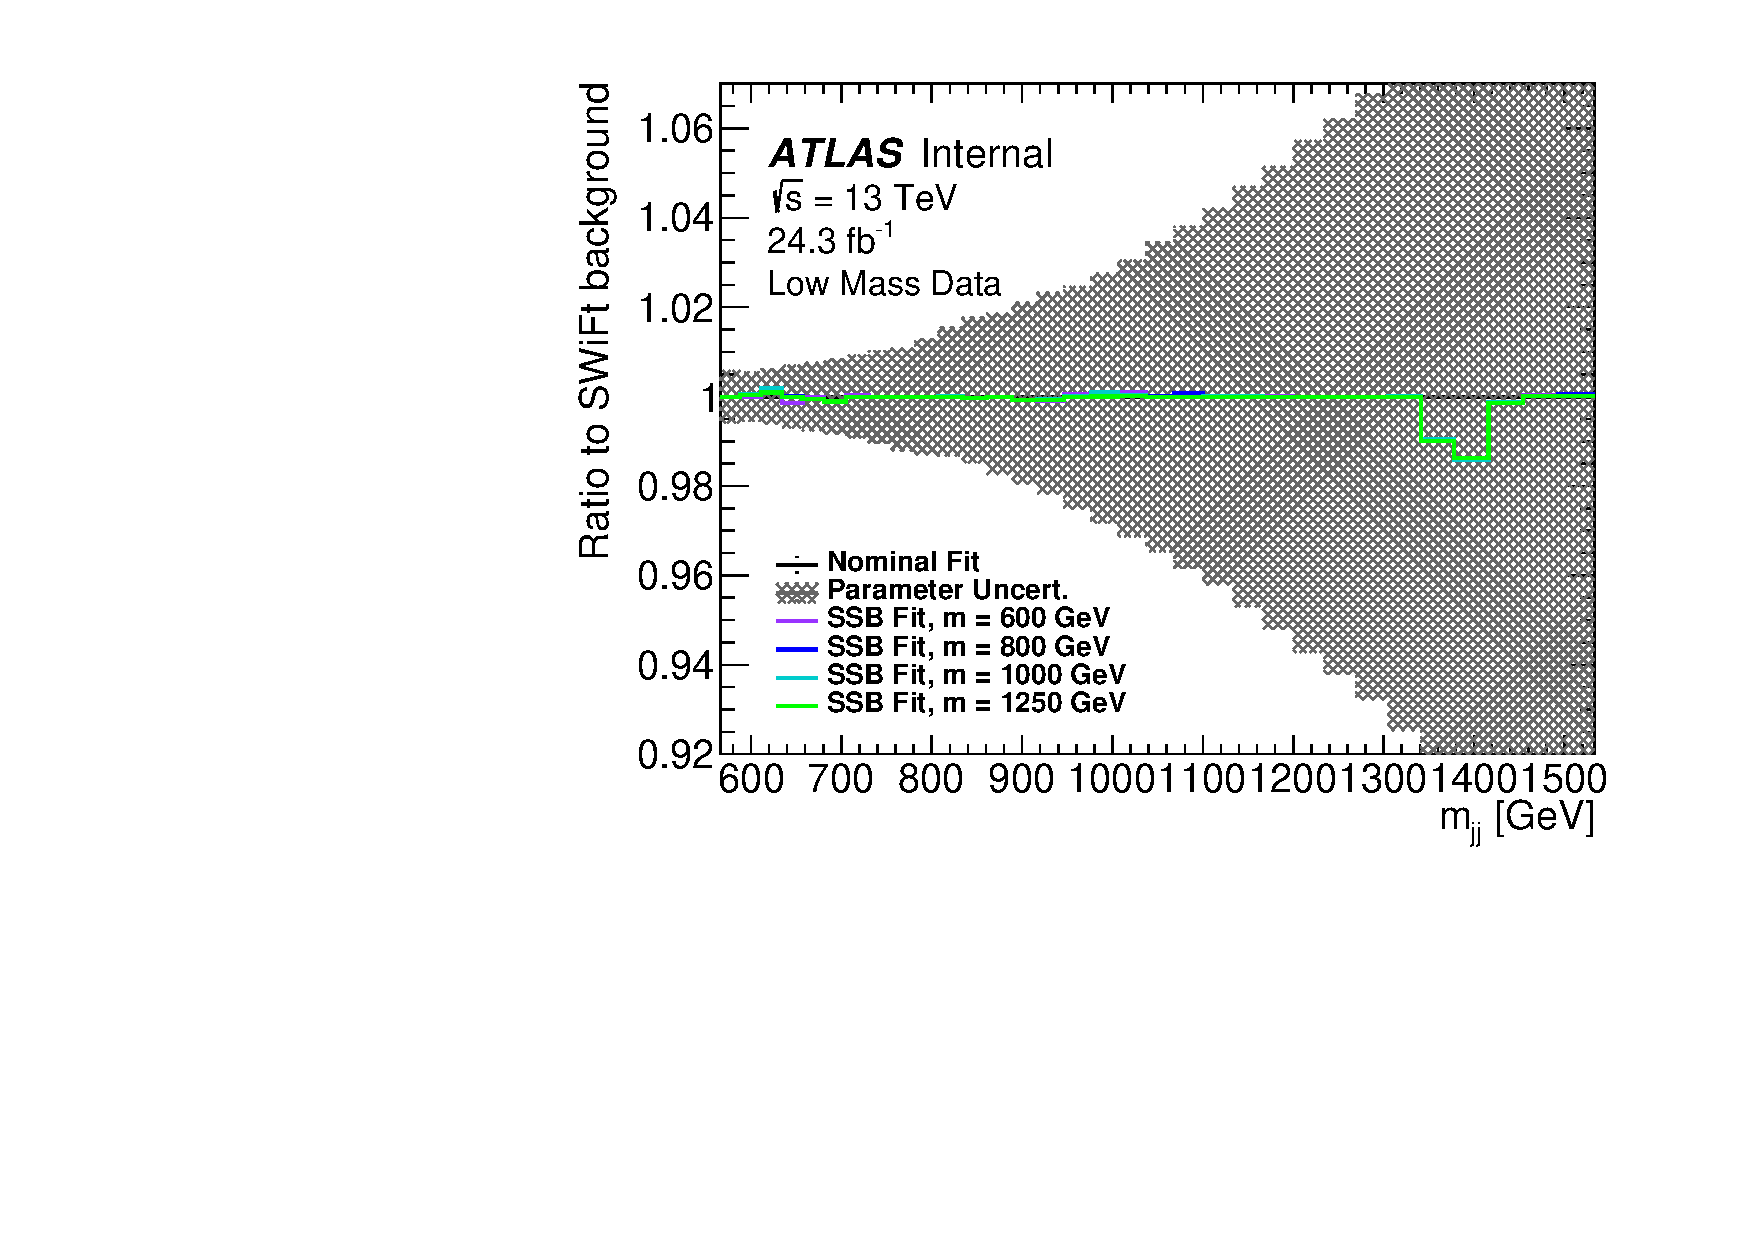
\includegraphics[width=0.6\linewidth, angle=0]{figs/Dibjet/LowMass/lim-ssb_data.pdf}
  \end{center}
  \vspace{-1mm}
  \caption{The ratio of signal subtracted background (SSB) estimations (coloured lines)
    and the SWiFt background estimate (black) performed on the full \lm{} data-set.
    The parameter choice uncertainty on the background is shown by the grey hashed area.
    The signal mass points used in the subtracted background estimations are indicated in the legend.}
  \label{fig:lim-lowmass_ssb_data}
\end{figure}

Finally, it is important to note that no signal plus background fit is considered in the search phase result,
as this would mean that the search phase result is not model independent.
However, it is clear that the nominal SWiFt background estimation can be affected by a signal induced fit bias,
as shown in Figure~\ref{fig:lim-lowmass_ssb_test}.
As a result the sensitivity of the search phase is reduced to specific signal models relative to the results of the limit-phase presented below;
the reduced sensitivity is accepted to maintain model independence.

\subsection{Results}
\label{sec:lim-full_results}

%Figure~\ref{fig:lim-summer_zprime} and \ref{fig:lim-summer_bstar} show the %% When there was two
Figure~\ref{fig:lim-lowmass_benchmark} shows the
95\% credibility level upper limits set on $\sigma\,\text{x}\,\mathit{A}\,\text{x}\,\epsilon$
as a function of simulated mass for the $Z'$-boson .
%The signal models considered are described in Section~\ref{sec:evt-s+b}.
The observed limit, the expected limit and the 1 and 2 $\sigma$ uncertainty bands on the expected limit are shown.
Overlaid are theoretical predictions of $\sigma\,\text{x}\,\mathit{A}\,\text{x}\,\epsilon$ for the
Sequential Standard Model (SSM), leptophobic and DM $Z'$ boson benchmark models, which have been described in Section~\ref{sec:evt-s+b}.
These limits have not yet been published and can be considered as preliminary.

Using the \lm{} data-set it is anticipated that the SSM and leptophobic $Z'$-boson
will be excluded in the simulated mass range 0.6-1.25 TeV at the 95\% credibility level.
Additionally it is anticipated the DM $Z'$-boson will be excluded in the simulated mass range
0.6-0.95 TeV  at the 95\% credibility level.

\begin{figure}[!ht]
  \centering
  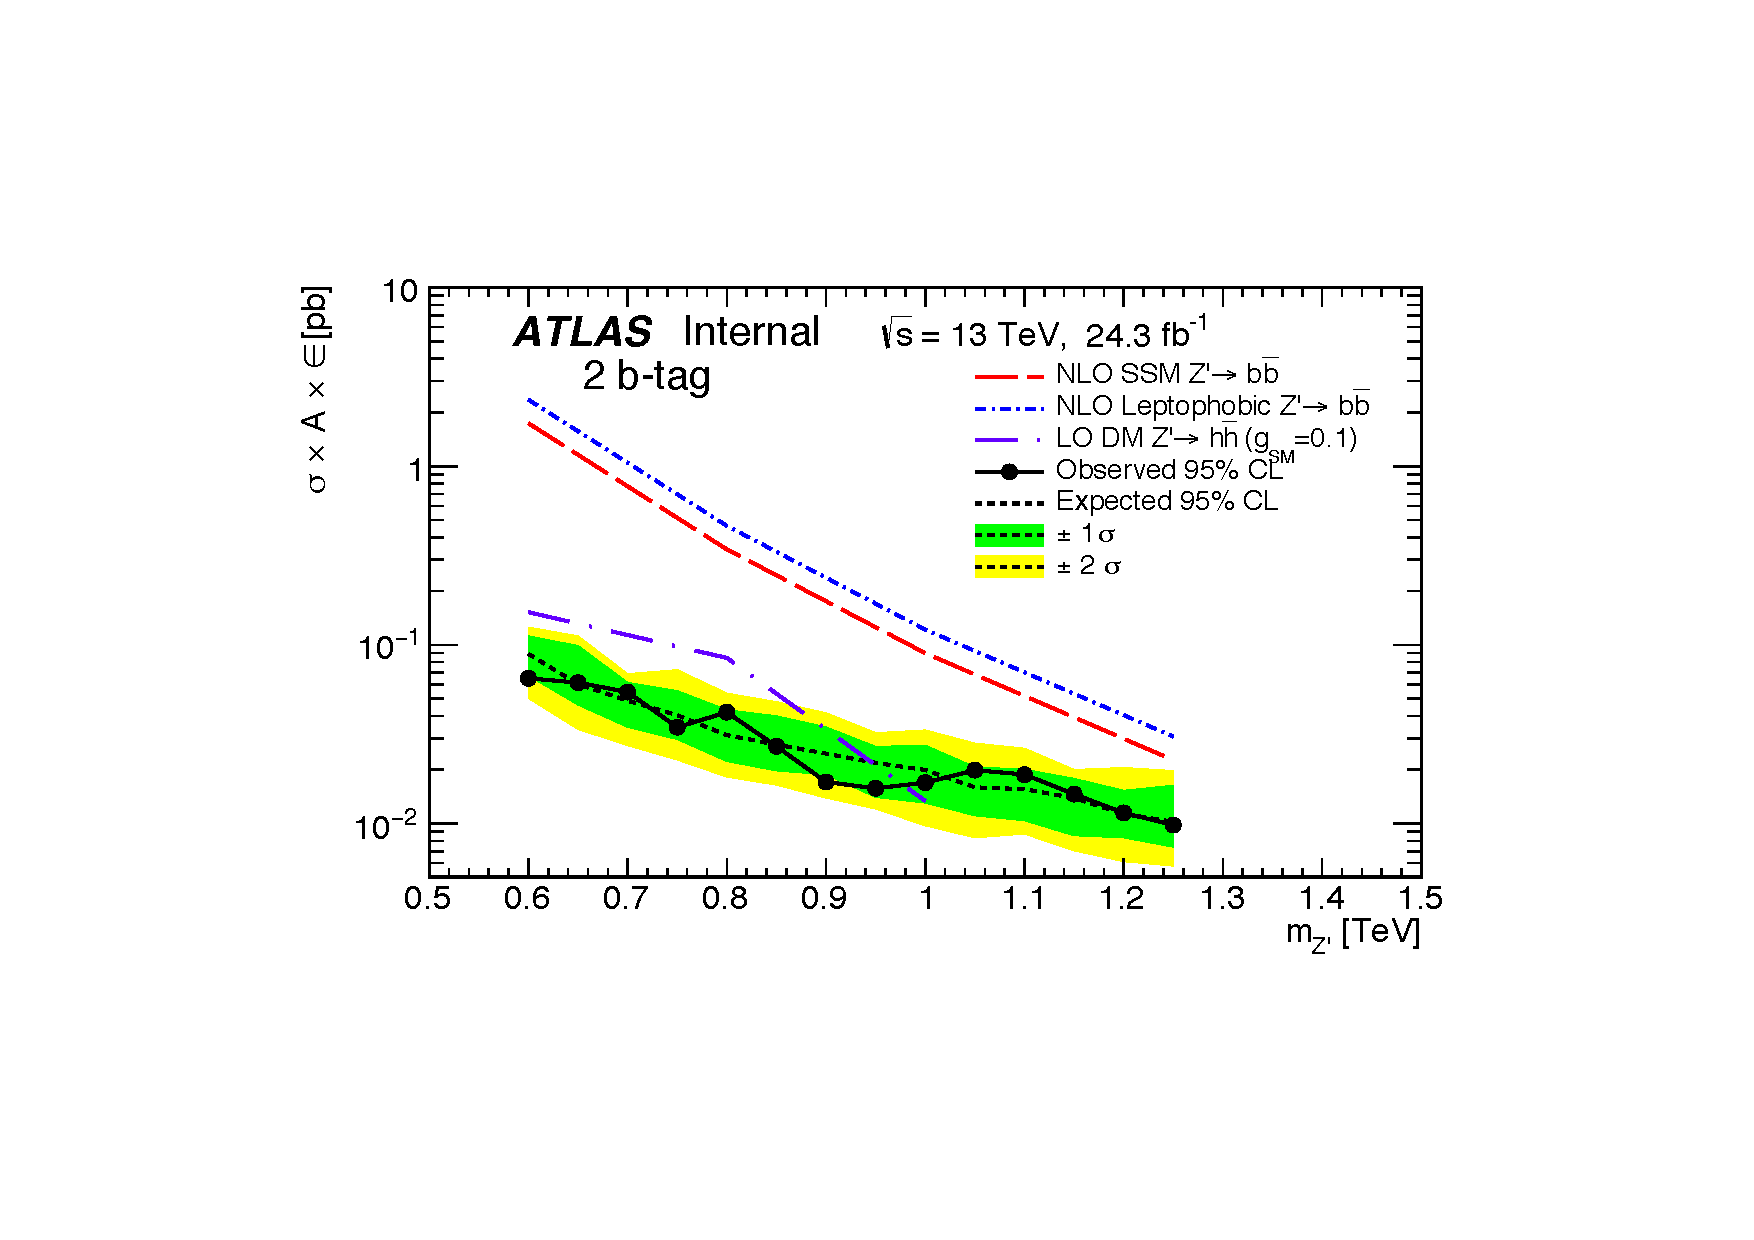
\includegraphics[width=0.8\linewidth, angle=0]{figs/Dibjet/LowMass/lim-zprime.pdf}
  \caption[Bayesian 95\% credibility level upper limits on
           cross-section times acceptance times tagging efficiency
           ($\sigma\,\text{x}\,\mathit{A}\,\text{x}\,\epsilon$)
           for the $Z'$-boson and as a function of simulated mass using the \lm{} data-set.
           The observed limit is shown by the solid black line, the expected limit is shown by the dotted black line
           and the 1 and 2 $\sigma$ uncertainty bands on the expected limit are shown by the green and yellow bands.
           The theoretical prediction of $\sigma\,\text{x}\,\mathit{A}\,\text{x}\,\epsilon$
           for the Sequential Standard Model (SSM), leptophobic and DM $Z'$-bosons are overlaid.]
          {Bayesian 95\% credibility level upper limits on cross-section times acceptance times tagging efficiency
            ($\sigma\,\text{x}\,\mathit{A}\,\text{x}\,\epsilon$)
             for the $Z'$-boson and as a function of simulated mass using the \lm{} data-set.
             The observed limit is shown by the solid black line, the expected limit is shown by the dotted black line
             and the 1 and 2 $\sigma$ uncertainty bands on the expected limit are shown by the green and yellow bands.
             The theoretical prediction of $\sigma\,\text{x}\,\mathit{A}\,\text{x}\,\epsilon$
             for the Sequential Standard Model (SSM), leptophobic and DM $Z'$-bosons are overlaid~\cite{dibjet-full_int}.}
  \label{fig:lim-lowmass_benchmark}
\end{figure}


For the generic Gaussian limit setting procedure there is a significant difference
with respect to the \summer{} data-set analysis.
In the \summer{} data-set analysis a signal template with a Gaussian distribution in dijet mass is used,
whilst for the \lm{} data-set analysis a signal template with a Gaussian distribution in the truth mass distribution is used.
The truth mass is defined as the invariant mass of the leading and subleading truth jets,
using the definition of truth jet from Section~\ref{sec:obj-jets_calib}.
The Gaussian shapes are centred on a range of simulated masses and the width of the considered Gaussians are
15\%, 10\%, 7\%, 5\%, 3\% and 0\% of the simulated mass;
a Gaussian with a 0\% width is a Dirac delta peak.
The transformation of the signal templates from truth mass to dijet mass is performed using
transfer matrices calculated using Monte-Carlo simulated QCD dijet samples,
following the procedure outlined in~\cite{dijet-mori17_paper}.
The Gaussian with a 0\% width in truth mass will have
a width of the mass resolution of the detector in dijet mass.

For the Gaussian limit setting the sources of systematic uncertainties
are the luminosity uncertainty,
the background modelling uncertainties and a flat 5\% uncertainty to cover
the JES, JER and $b$JES systematic uncertainties.
Other systematic are not included in the preliminary Gaussian limit
as uncertainties are found to have a small effect on upper limit relative to the resolution uncertainties,
as these can significantly broaden the width of the dijet mass signal template.

Figure~\ref{fig:lim-lowmass_gauss} shows the observed 95\% credibility upper limits set 
on the product of cross-section, detector acceptance, tagging efficiency and branching ratio,
$\sigma\,\text{x}\,\mathit{A}\,\text{x}\,\epsilon\,\text{x}\,\mathit{BR}$,
for the full range of Gaussian signals described above.
The expected limits for a Gaussian signal with a 0\% width
in simulated mass is shown by the dotted lines and associated 1~and~2~$\sigma$ uncertainty bands
are shown in green and yellow.
The results have not yet been published and can be considered as preliminary.

For the \lm{} data-set it is anticipated that an upper limit will be placed
on a generic Gaussian signal ranging from 0.05 to 0.003 pb in the mass range 0.65 to 1.4 TeV.

\begin{figure}[!ht]
  \begin{center}
    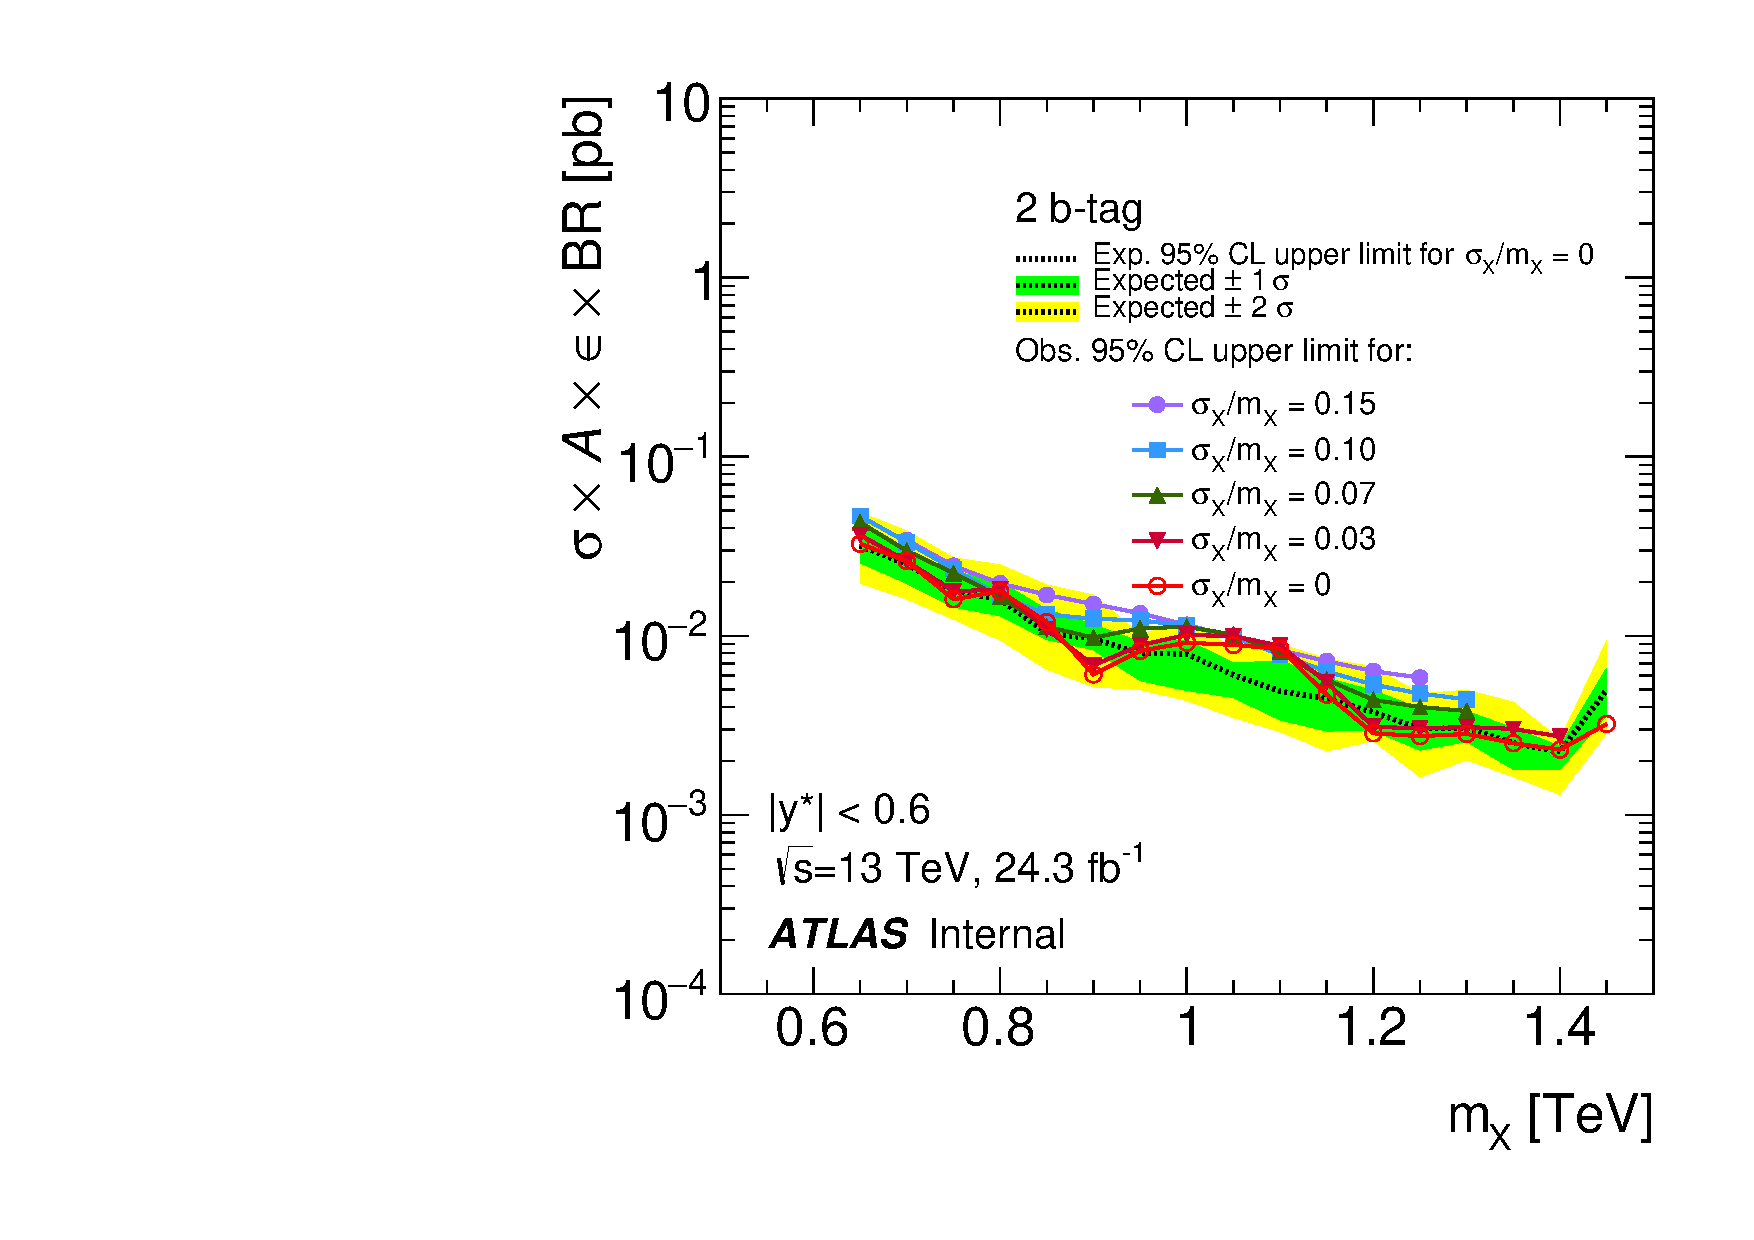
\includegraphics[width=0.6\linewidth, angle=0]{figs/Dibjet/lowmass/lim-gaussian.pdf}
  \end{center}
  \caption[95\% credibility upper limits
    on the product of cross-section, detector acceptance, tagging efficiency and branching ratio,
    $\sigma\,\text{x}\,\mathit{A}\,\text{x}\,\epsilon\,\text{x}\,\mathit{BR}$,
    for Gaussian signals using the \lm{} data-set.]
  {95\% credibility observed upper limits
    on the product of cross-section, detector acceptance, tagging efficiency and branching ratio,
    $\sigma\,\text{x}\,\mathit{A}\,\text{x}\,\epsilon\,\text{x}\,\mathit{BR}$,
    for Gaussian signals using the \lm{} data-set are shown by the solid lines.
    The signal templates are Gaussian in simulated mass with
    widths of 15\%, 10\%, 7\%, 5\%, 3\% and 0\% of the simulated mass.
    Also shown are the expected 95\% credibility observed upper limit on the Gaussian signal shape with a 0\% width (dotted line)
    and the associated 1~\sigma\ and 2~\sigma{} (yellow and green bands)~\cite{dibjet-full_int}.
  }
  \label{fig:lim-lowmass_gauss}
\end{figure}
